% !Mode:: "TeX:UTF-8" 

\BiChapter{克隆代码变化一致性维护需求预测方法}
{Predicting Clone Changing Consistency-Requirement in A Clone Group}

\BiSection{引言}
{Introduction}

本文第3章研究克隆创建时的一致性维护需求预测,可帮助程序开发人员避免会导致额外维护代价的克隆代码。但是,软件系统中已经存在相当数量的克隆代码,其可能会被开发人员修改而导致一致性变化,遗忘这种一致性变化会引入克隆一致性违背缺陷。针对软件中已存在的克隆代码,在克隆代码发生变化时(被开发人员修改时),预测该变化是否会引发其所在克隆组的一致性维护,可以避免由于遗忘该变化而导致的克隆代码一致性违背缺陷。因此,在克隆代码变化时如何预测克隆代码的一致性维护需求是一个值得研究的问题,可以帮助提高软件质量和可维护性。

第3章克隆代码一致性维护的目的是为了规避可能导致额外维护代价的克隆代码产生,关注的是由复制粘贴操作产生的新的克隆代码,所提取的属性特征也与复制粘贴操作相关。而本章克隆代码一致性维护的目的是为了避免克隆代码一致性变化的一致性违背缺陷,关注的是发生变化的克隆代码,因需求和关注点不同从不同的角度提取了不同的属性特征。首先,通过构建软件系统的克隆家系,并识别来收集系统中所有的克隆变化实例(发生变化的克隆组)。然后,提取了代码属性、上下文属性描述发生变化的克隆组,并新增一组演化属性描述其历史演化情况。最后,训练机器学习模型预测克隆代码变化的一致性维护需求。在四个开源软件系统上对本章方法进行了评估,实验结果表明本章方法可以有效地预测克隆代码变化一致性维护需求。本章的预测方法可以帮助开发人员在克隆代码变化时预测克隆代码的一致性,避免克隆变化导致的一致性违背缺陷。

\BiSection{克隆代码一致性维护的相关研究}
{Related Work for Code Clone Consistency-Maintenance}

\BiSubsection{克隆变化对软件质量影响的问题}
{The Clone Change Effect for Software Quality}

克隆代码不仅可能会导致额外的维护代价,更重要的是还有可能引发相关缺陷。首先,发生一致性变化的克隆代码会增加了软件的额外维护代价;其次,如果忘记对需要一致性变化的克隆代码进行一致性维护,会向系统中引入克隆一致性违背缺陷(Consistency Defect)\cite{bettenburg2009empirical,juergens2009code}。

给出系统jEdit中存在的克隆代码一致性变化示例,如图~\ref{changingexamplea}~和~\ref{changingexampleb}~所示。图~\ref{changingexamplea}~中给出了$ 3.1.0 $版本中的两个克隆代码片段。在随着系统演化至$3.2.0$版本时,上述两个克隆代码发生了一致性变化。如图~\ref{changingexampleb}~所示,$ 3.1.0 $版本中的第9 - 12行和第15行代码在版本$ 3.2.0$中被开发人员修改。第9 - 12行,开发人员将{selectionEnd}更改为$0$,并删除了一对花括号。在第15行,开发人员删除了声明语句。开发人员对上述两个克隆代码进行了一致性维护,从而避免了克隆代码的一致性违背缺陷。

\begin{figure}[htbp]
\centering
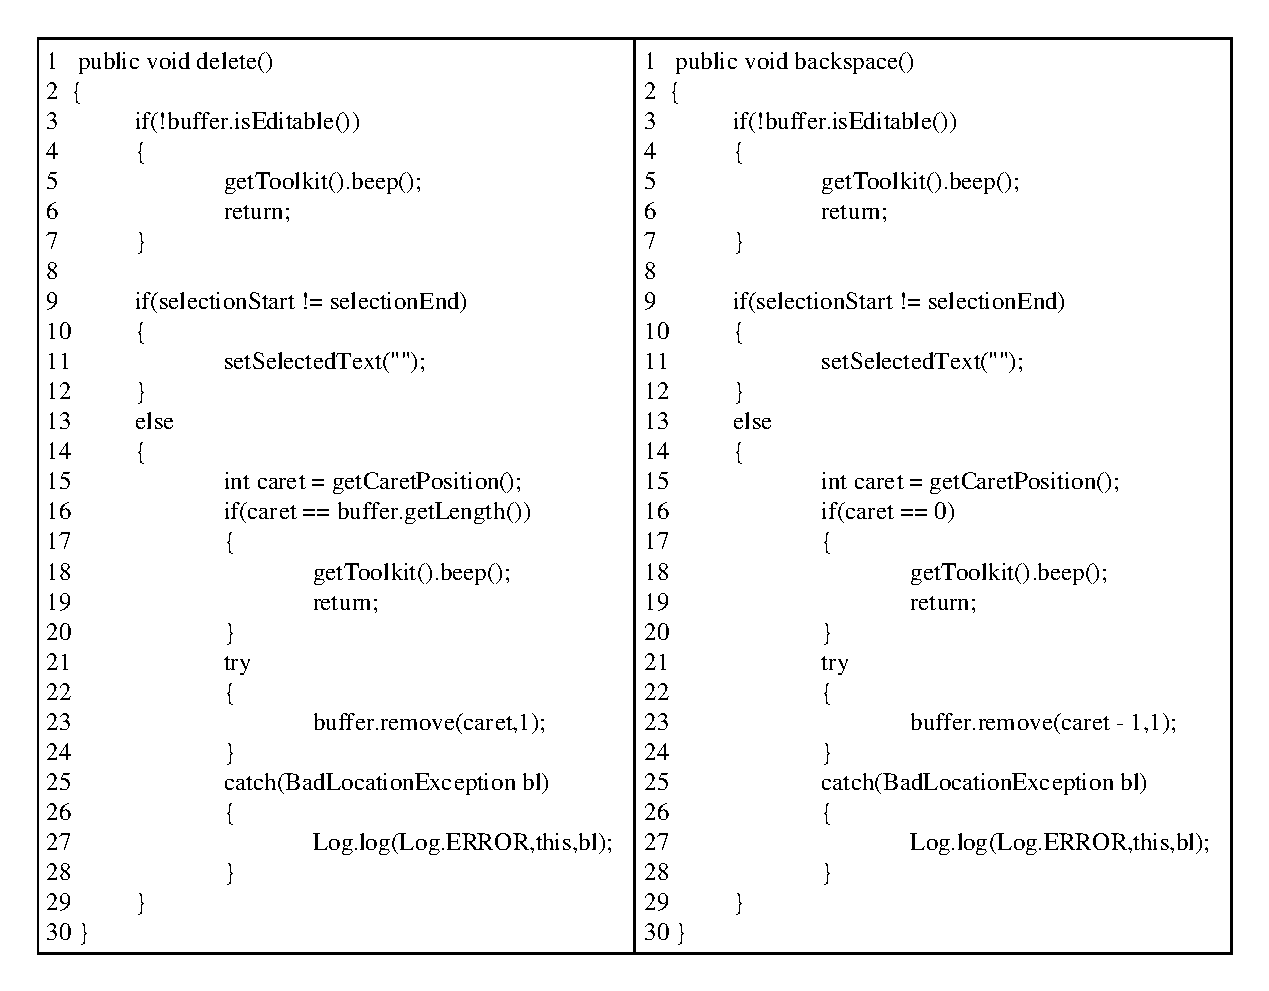
\includegraphics[width=0.8\textwidth]{co-changea.pdf}
\bicaption[changingexamplea]{}{版本$ 3.1.0 $中未发生一致性变化前的同组克隆代码}
{Fig.$\!$}{Two clone fragments in one clone group before consistent change in version $3.1.0$}
\vspace{-1em}
\end{figure}

\begin{figure}[htbp]
\centering
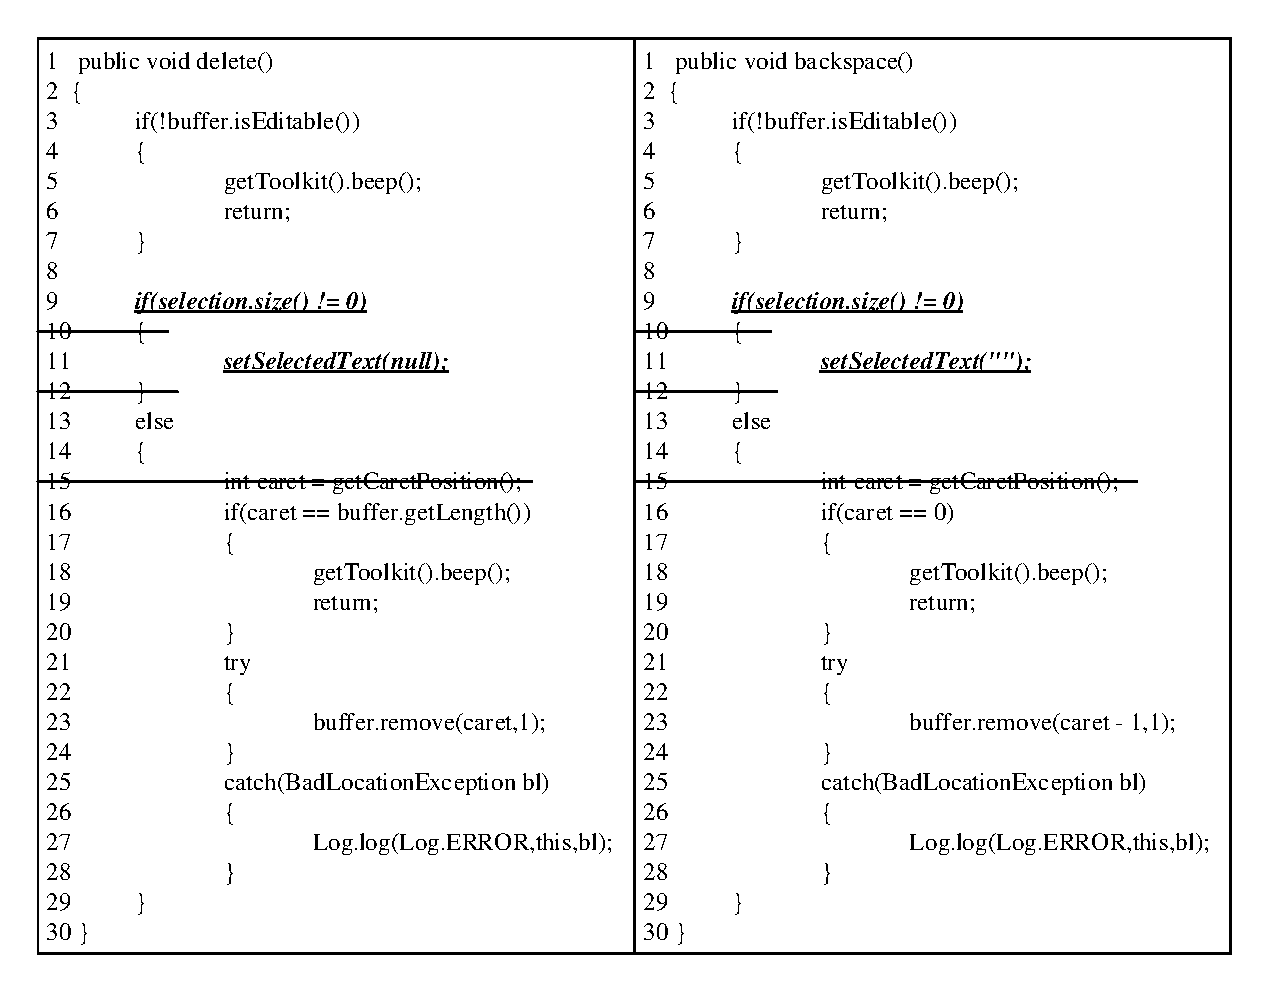
\includegraphics[width=0.8\textwidth]{co-changeb.pdf}
\bicaption[changingexampleb]{}{版本$ 3.2.0 $中发生一致性变化后的同组克隆片段}
{Fig.$\!$}{Two clone fragments in clone group after consistent change in version $3.2.0$}
\vspace{-1em}
\end{figure}

图~\ref{changingexamplec}~是会导致一致性违背缺陷的克隆代码示例。图中Clone A是一段代码,将数量为nRegs的内存数据转移值数组ppTotal中。程序开发人员将Clone A复制并粘贴至另一个位置成为Clone B。Clone B具有相似的功能,将数量为nRegs的内存数据转移值数组ppTaken中,并将代码中的ppTotal重命名为ppTaken。在随后的演化中,发现Clone A存在潜在的边界问题,并在第5行添加条件语句{if (i+1<nRegs)},将其修改为 Clone A'。代码Clone B也需要添加相似的判断语句,然而遗憾的是开发人员遗忘了该一致性变化,导致Clone B'中存在一个一致性违背缺陷。因此,开发人员未能在需要时对克隆代码进行一致性维护,会导致了克隆代码的一致性违背缺陷,并降低软件的质量、增大其维护代价。

\begin{figure}[htbp]
\centering
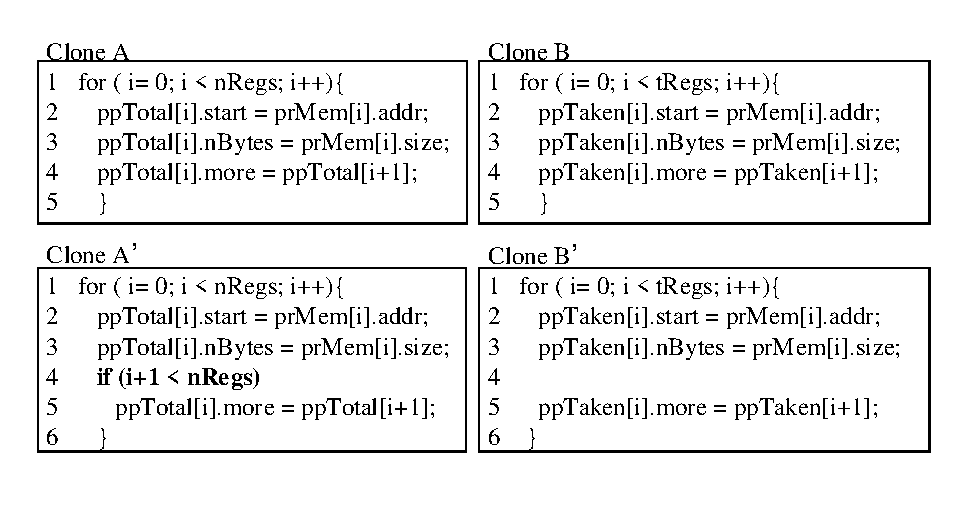
\includegraphics[width=0.7\textwidth]{co-changec.pdf}
\bicaption[changingexamplec]{}{导致一致性违背缺陷的克隆代码\cite{nguyen2012clone}}
{Fig.$\!$}{An example for code clones that resulting consistency defect\cite{nguyen2012clone}}
\vspace{-1em}
\end{figure}

\BiSubsection{现有研究存在的问题}
{Problems in Current Research}

在克隆代码随着软件系统进行演化的过程中,克隆组内的某一克隆代码片段可能会被程序开发人员修改,并引发克隆代码的一致性变化\cite{saha2011automatic}(如图~\ref{changingexamplea}~和~\ref{changingexampleb}~所示)。对于需要一致维护的克隆代码变化,如果遗忘克隆的一致性变化,会导致克隆代码的一致性违背缺陷\cite{aversano2007clones,bettenburg2009empirical}(如图~\ref{changingexamplec}~所示)。

为了维护演化中的发生变化的克隆代码,研究人员进行了克隆代码一致性维护的研究。Cheng等人提出了一个基于Token的克隆代码一致性维护方法,当克隆组内的一个代码发生变化时,能够同时修改组内的其他克隆代码,保证克隆代码的一致性\cite{cheng2016rule}。但是,该方法未对克隆代码是否需要一致性维护进行判定,缺少必要的先行条件。同时,克隆管理工具JSync也支持克隆代码的一致性维护\cite{nguyen2012clone}。但是,该方法仅能支持标识符的一致性维护,也未在发生变化时对克隆代码进行一致性维护的判断。Yamanaka等人将克隆变化与事件通知机制相结合,将每一个克隆变化都看成一个事件,在克隆发生变化时提醒开发人员及时地对克隆变化进行维护\cite{yamanaka2013applying}。但是,该方法会将所有的克隆代码变化通知开发人员,也没有区分对是否需要一致性维护进行判定,仍需开发人员手工验证。Mondal等人通过对克隆组内的克隆代码排序,从而预测需要一致性维护的克隆代码\cite{mondal2014prediction}。但并不是在克隆代码发生变化时进行预测,无法实时的帮助维护克隆代码。Murakami等人在克隆代码未发生变化时,预测克隆代码是否会发生下一次变化\cite{murakami2014predicting}。该方法仅仅预测了是否会发生变化,既没有在变化发生时进行预测,也没有区分克隆代码的一致性和不一致性变化。

现有对克隆代码变化维护研究依然存在以下两点不足之处:

(1)现有的克隆代码一致性维护研究中,假定需要一致性维护的克隆代码是已知的,即已知哪些克隆代码是需要一致性维护的。在此假设条件下,研究克隆代码一致性维护方法,即如何维护此类克隆代码保证其变化的一致性。因此,当前的研究中,缺少对发生变化的克隆代码是否需要一致性维护的判定研究。

(2)现有的克隆变化的预测方法中,仅预测哪些克隆代码会发生变化,既没有预测克隆代码发生变化的时刻,也没有预测其是否需要一致性的维护。因此,预测结果不能指导开发人员对发生变化的克隆代码进行一致性维护。

综上所述,当软件中的克隆代码发生变化时,由于克隆组内的克隆片段的相似性可能会引发一致性变化,遗忘一致性变化会导致克隆代码的一致性违背缺陷。因此,预测克隆代码变化的一致性维护需求是一个值得研究的问题,可以帮助开发人员避免一致性违背缺陷,并提高软件质量和可维护性。具体来说,如果克隆代码的变化需要一致性维护,警告软件开发人员对变化所在的克隆组进行维护,从而避免一致性违背缺陷;如果克隆代码的变化不会引发一致性变化,则帮助开发人员可以更加自信的修改克隆代码,更快地对软件开发和维护。

\BiSubsection{本文的解决思路}
{The Proposed Method}

为在克隆代码克隆变化时避免其可能导致的一致性违背缺陷,本章将预测克隆变化的一致性维护需求。首先,定义克隆变化时的克隆代码一致性变化以及一致性维护需求。然后,对于发生变化的克隆代码,从其所在的克隆组的角度分别提取了代码属性和上下文属性表示该克隆组,从演化的角度提取了该克隆组的历史演化特征。最后,构建克隆变化的预测模型并预测克隆变化的一致性维护需求。本章方法可以帮助程序开发人员避免克隆一致性缺陷,提高软件的质量和可维护性。

本章的克隆变化一致性维护需求预测方法如图~\ref{framwork3}所示。从图中可以看出,该方法可以划分为三个阶段,克隆变化实例收集阶段、克隆变化实例表示阶段和一致性维护需求预测阶段。收集阶段旨在收集系统中全部的发生变化的克隆代码,可将其用于使用机器学习方法中来训练预测模型。首先,使用NiCad来检测软件版本中的所有克隆,并通过在相邻版本的克隆组之间进行映射来构建克隆家系。然后,并通过分析所映射的克隆组之间的克隆演化模式(一致性变化模式),从而收集系统中发生变化的克隆代码,并将该克隆组标记为克隆变化实例。最后,通过遍历克隆家系中的演化模式从软件中收集全部的克隆变化实例。

\begin{figure}[htbp]
\centering
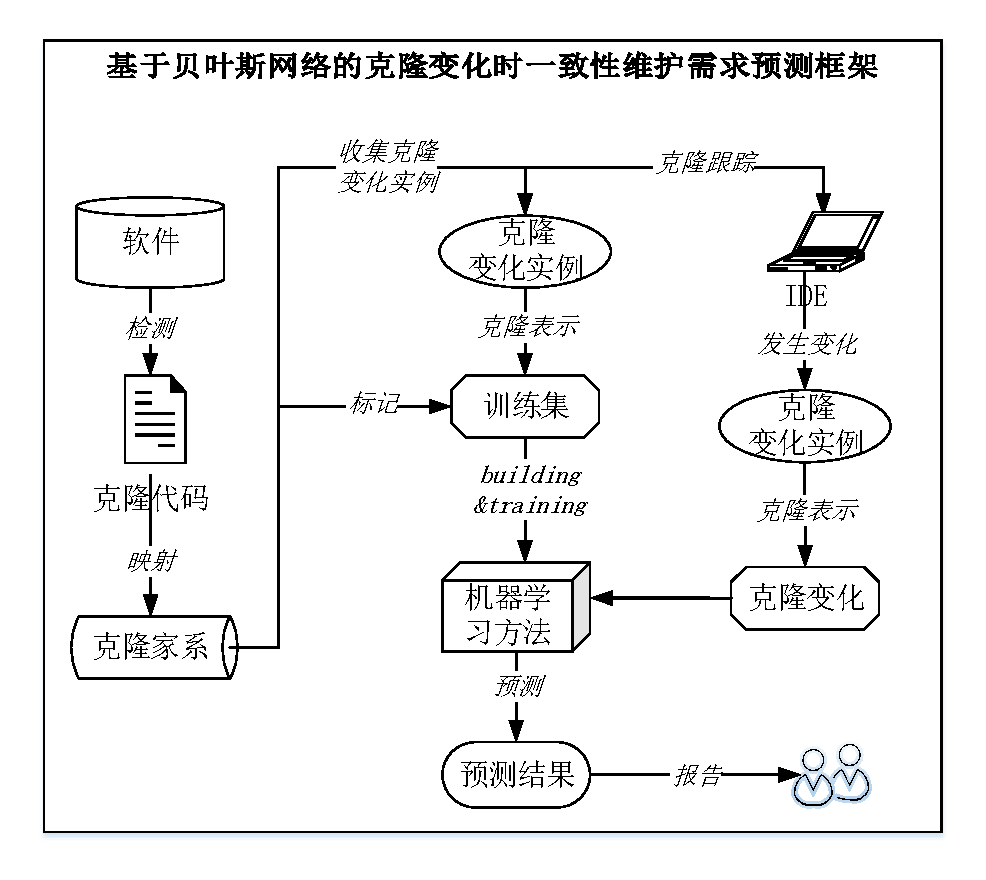
\includegraphics[width = 0.7\textwidth]{framework4.pdf}
\bicaption[framework4]{}{克隆代码变化一致性维护需求预测方法}
{Fig.$\!$}{The approach for clone changing consistency prediction}
\vspace{-1em}
\end{figure}

在克隆变化表示阶段中,将提取相应的属性值表示克隆变化实例。与第3章不同的是,将从克隆组的角度提取代码属性、上下文属性,并新增演化属性一共三组属性组表示克隆变化实例。同时,还提取了关于克隆变化的相关信息,用于描述此次发生的变化。

在预测阶段中,使用收集到的克隆变化实例训练机器学习模型,并在克隆变化时预测克隆一致性维护需求。程序开发人员根据预测结果,可以采取不同的操作。对于会导致一致性变化的克隆代码变化,其在将来的演化中可能会引发缺陷。因此,需要通知程序开发人员检测整个克隆组的一致性。对于不会导致一致性变化的克隆代码变化,其不会引发克隆一致性违背缺陷。因此,在程序开发人员可以放心的对该克隆代码进行修改,不必考虑克隆代码的一致性问题。

本章针对软件中存在的发生变化的克隆代码,预测其一致性维护需求,将重点分析讨论如下问题:

(1)在克隆代码发生变化时(克隆片段被修改时),结合其可能导致的克隆一致性违背缺陷,如何描述和定义克隆代码的一致性变化和一致性维护需求?

(2)对于克隆变化实例(发生变化的克隆组),如何描述和表示发生变化的克隆组及其所发生的变化?

(3)在预测克隆变化一致性维护需求时,如何结合软件开发过程帮助程序开发人员避免可能导致的一致性违背缺陷?

\BiSection{克隆代码变化时一致性维护需求的定义}
{The Definitions for Clone Changing Consistency-Requirement}

在第3章中,本文给出了一个克隆代码创建时的一致性变化模式定义。但是,当预测克隆代码变化时的一致性维护需求时,该定义仅仅要求同一克隆组克隆代码片段发生变化,并没有限制发生什么样的变化。该定义无法应用于本章克隆代码变化时的一致性维护需求预测中。因此,对克隆变化时的一致性变化模式进行了重新定义,如下所示:

\begin{definition}[克隆变化时一致性变化模式] 
\label{def-changingpattern}
在软件版本 $j+1$中存在一个克隆组$CG'$ ,假设克隆组内至少存在两个克隆代码片段$CF'_1$ 和 $CF'_2$可以与映射到上一版本$j$的克隆组$CG$中,且 $CG$中与之对应的克隆代码片段的 $(CF_1,CF_2)$被修改为$(CF'_1,CF'_2)$。如果对于一个的接近于0的阈值$\tau$,克隆代码$CF_1$和$CF_2$的变化满足:
\begin{equation}
\begin{split}
  \begin{array}[t]{crl}
    \mathit{TextSim}(CF_i, CF'_i) < 1 & \forall i \in \{1,2\} &(1) \\
    \multicolumn{2}{c}{| ~\mathit{TextSim}(CF_1,CF'_1)  ~-~ \mathit{TextSim}(CF_2,CF'_2) ~| ~< ~ \tau}  & (2)
  \end{array}
\end{split}
\end{equation}
则称克隆组$CG'$具有克隆变化一致性变化模式(Changing Consistent Change Pattern)。
\end{definition}

在该定义中,克隆代码的变化同样使用$\mathit{TextSim}(CF_i, CF'_i)= 1 - \mathit{UPI}(CF_i, CF'_i)$定义。其中,UPI(Unique Percentage Items)表示两个代码片段之间不同的代码行数占总代码行的比例。在克隆代码变化时,不仅要求克隆代码片段被同时修改,还要求发生相同的变化,即克隆代码的变化包含两个约束条件。第一个约束条件要求 $CF_1 $和$CF_2 $同时被修改,第二个约束条要求$CF_1 $和$CF_2$发生相同的变化。在第二个约束条件中,一致性变化使用一个接近于0的阈值$\tau$限定,要求克隆片段发生了完全一致的修改。

要求发生相同变化的原因在于:在克隆代码变化时,本章的目的是避免由于克隆变化可能导致的克隆一致性违背缺陷。因此, 不仅要求两个克隆代码片段同时变化,还需要发生相同的变化。假如软件开发人员遗忘该变化,将会引入克隆一致性违背缺陷。

同第3章相似,本节定义的克隆组的一致性变化模式,也只要求至少存在两个克隆代码片段同时发生相同的变化。其原因在于:即使发生变化的克隆组有多于两个以上的克隆代码片段,仅有两个克隆代码变化的一致性变化,也可能会导致一致性违背缺陷。若要求组内全部的克隆片段发生相同的变化,将无法预测此类缺陷的发生。

本文将发生变化的克隆组称为克隆变化实例,通过识别克隆家系中的一致性变化模式,也可以获得软件中的发生变化的克隆代码(克隆变化实例)。克隆变化实例的定义如下所示:

\begin{definition}[克隆变化实例] 
\label{def-changinginstance}
软件版本 $j$中的一个克隆组$CG$是克隆变化实例,如果克隆组$CG$中至少两个克隆代码片段发生变化,且版本$j+1$ 中至少存在一个克隆组$CG'$与之对应(在同一克隆家系$CGE$中)。 
\end{definition}

为更好的理解发生变化的克隆代码,即克隆变化实例。现给出一个克隆组的克隆家系以及克隆变化实例,如图~\ref{changinggena}~所示。如图所示,图中给出一个克隆组$CG$的克隆家系,该克隆组在版本$j$到$j+1$的演化过程中,克隆代码片段发生了变化,因此克隆组$CG_j$是一个克隆变化实例。值得注意的是,该变化可能是一致性变化也可能是不一致性变化。

\begin{figure}[htbp]
\centering
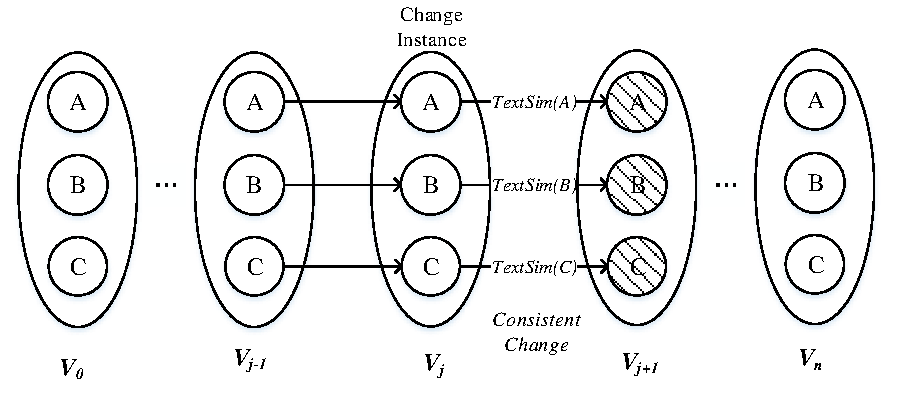
\includegraphics[width = 0.6\textwidth]{changinggena.pdf}
\bicaption[changinggena]{}{克隆变化实例示意图}
{Fig.$\!$}{An example for clone changing instance}
\vspace{-1em}
\end{figure}

当演化中的克隆代码变化时,其所在的克隆组是一个克隆变化实例,该变化可能会导致克隆组的一致性变化,进而可能引发克隆一致性违背缺陷。假设在克隆代码变化时预测其是否会导致一致性变化,则帮助避免一致性违背缺陷。因此,本文将克隆变化所导致的一致性变化,称为克隆变化一致性维护需求,定义如下:

\begin{definition}[克隆变化时一致性维护需求] 
 \label{def-changingrequirement}
给定版本 $j$中一个克隆变化实例$CG$,如果在版本$k$中存在一个克隆实例 $CG'$($k>j$)满足以下条件: (1) 在$CG'$中至少存在两个克隆片段在其克隆家系$CGE$中可以映射到克隆实例 $CG$中, (2) $CG'$ 具有“变化时一致性变化模式”(Changing Consistent Change Pattern),则称克隆变化实例$CG$满足克隆变化的一致性维护需求(Changing Consistency-Requirement);反之,如果不存在一个克隆实例 $CG'$,称该克隆变化实例$CG$不需要一致性维护(Changing Consistency-Requirement Free,或Consistency-Free,或Free)。
\end{definition}

根据上面的定义,对于某一个克隆变化实例$CG_j$,假如其会导致一致性变化,要求在$CG_j$在未来的演化中发生一致性变化模式即可,而不是仅仅限定$CG_{j+1}$拥有一致性变化模式。原因在于:研究发现克隆代码的一致性变化可能具有延迟传播现象\cite{barbour2011late,mondal2016comparative}。延迟传播指克隆片段的变化没有立即传播到其所在的克隆组中,而在间隔一定数量的版本后传播,继续发生一致性变化。值得注意的是,本章的定义可以同时涵盖$CG_{j+1}$拥有一致性变化模式和可能发生延迟传播的情况。

根据上面的定义,本章的研究问题可以表述如下:给定一个克隆变化实例$CG$,即克隆组中$CG$的克隆代码片段$CF$被修改,确定$CG$是否满足克隆变化一致性维护需求。根据上述定义克隆变化实例只有两种状态:满足和不满足一致性维护需求。将变化实例的一致性要求的预测转化为分类问题。可以使用机器学习模型解决此分类问题。

\BiSection{克隆变化实例的获取}
{Collecting Clone Changing Instance}

收集克隆变化实例的目的在于生成克隆一致性维护需求预测的训练集,并将其用于训练机器学习模型。通过构建系统的克隆家系并识别其中的克隆演化模式,可以从软件中收集所有的克隆变化实例。根据定义~\ref{def-changinginstance}~,本文假定克隆家系$CGE$中发生变化的克隆组为克隆变化实例。因此通过构建克隆家系并识别克隆家系中发生变化的克隆组,可以收集克隆创建实例。

(1)构建克隆家系

首先,下载系统所有版本的源代码,并使用NiCad的默认配置检测检测每一版本的中Type1-3的克隆代码。然后,通过映射所有相邻版本的克隆代码,构建系统中全部克隆家系。为完成版本间的映射,为每个克隆片段生成一个克隆区域描述符 $CRD$\cite{duala2010clone},使用基于CRD的克隆映射算法映射两个连续版本之间的所有克隆片段和克隆组\cite{ci2013new,ci2013newD}。根据克隆映射结果,构建系统的克隆家系。

(2)识别克隆演化模式并收集克隆变化实例

首先,识别克隆家系中的克隆演化模式。构建克隆家系后,通过对比相邻版本的克隆代码,可以识别克隆家系的克隆演化模式,尤其是一致性变化模式(参考定义~\ref{def-evolutionpattern}~和\ref{def-changingpattern}~)。所识别的克隆演化模式有三个作用:(a)可以用于表示克隆变化实例,本文使用克隆演化模式作为表示克隆变化实例的部分演化属性。因此,克隆演化模式可以用于克隆变化实例表示中。(b)克隆演化模式可以帮助收集克隆变化实例。根据定义~\ref{def-changingpattern}~可以识别系统中发生一致性变化的克隆代码和克隆组,从而确定克隆家系中的克隆变化实例。(c)克隆演化模式可以帮助确认克隆一致性维护需求。根据定义~\ref{def-changingrequirement}~一致性维护需求,可以通过遍历克隆家系$CGE$是否发生了一致性变化模式(定义~\ref{def-changingpattern}~)进行确定。

然后,收集克隆变化实例。在识别克隆家系演化模式,尤其是一致性变化模式后(定义~\ref{def-changingpattern}~),根据定义~\ref{def-changinginstance}通过识别克隆家系中的变化克隆组,便可以收集系统中的克隆变化实例。

(3)标识克隆变化实例的一致性维护需求

在收集所有的克隆变化实例后,还需确认相关实例的一致性需求。根据定义~\ref{def-changingpattern}~和~\ref{def-changingrequirement}~,通过遍历克隆变化实例所在的克隆家系$CGE$的演化情况,确定其一致性维护需求。如果克隆变化实例在其演化过程中发生了一致性变化模式(定义~\ref{def-changingpattern}~),则该实例满足一致性维护需求,否则不满足维护需求。

克隆创建实例收集算法如~\ref{alg-collectionchanging}~所示。算法中第1 - 5行是为克隆代码生成CRD,并使用CRD映射相邻版本的克隆代码,并根据克隆演化模式定义,识别克隆演化模式。假设一个版本中有$m$个克隆代码,生成CRD所需时间为$O(m)$,$n$个版本所需时间为$O(m*n)$。映射克隆相邻版本的克隆代码时间复杂度为$O(n)$。第6行是生成系统的克隆家系。第7 - 9行,收集克隆变化实例并标识其一致性维护需求。首先,根据克隆家系中的一致性变模式化,收集克隆变化实例。然后,根据克隆变化实例的后续演化过程中的克隆组的是否发生一致性变化,标记其一致性维护需求。算法复杂度为$O(n)$。所以,该算法的复杂度为$O(m*n)$。

\vspace{1em}
\begin{minipage}{0.8\textwidth}
\centering
\begin{algorithm}[H]
\AlgoBiCaption{克隆变化实例收集算法} {Algorithm for collecting clone changing instances}
\label{alg-collectionchanging}
\KwIn{All source code and code clones from $N$ versions}
\KwOut{All the clone changing instances}
\For{$i$=1 to $N$}
{ 
 Generating CRD to represent each code clone {CFs}\;
 Mapping all the $CFs$ and $CGs$ between the adjacent versions {i} and {i+1}\;
 Identifying all clone evolution pattern in thus two versions according to Definition~\ref{def-evolutionpattern}~\;
 Identify all clone consistent change pattern in thus two versions according to Definition~\ref{def-changingpattern}~\;
}
Generating all clone genealogies $CGEs$ with number $N\_cge$\;
\For{$i$=1 to $N\_cge$}
{ 
 Collecting the clone changing instance from $CGE\_i$ according to Definition~\ref{def-changinginstance}~\; 
 Labeling its consistency-requirement according to Definition~\ref{def-changingrequirement}~;
}
\Return {All clone changing instances\;}
\end{algorithm}
\end{minipage}
\vspace{1em}

\BiSection{克隆变化实例的特征描述}
{The Attributes for Clone Changing Instance}
\label{lab-changingattribute}

本章使用机器学习中分类方法预测克隆代码变化的一致性维护需求,并使用软件中既有的克隆变化实例训练不同的机器学习模型。但是,实际的克隆变化实例无法直接应用于机器学习中。因此,本节将提取相应的属性值表示克隆变化实例。对于一个克隆变化实例,其本质上是一个发生变化的克隆组。对于该发生变化的克隆组,将从克隆组的角度分别提取代码属性特征、上下文属性特征和演化属性特征描述该克隆变化实例。值得注意的是,克隆变化实例的代码属性和上下文属性与本文第3章中克隆创建实例的属性不同,区别在于克隆变化实例将从克隆组的角度提取相应的属性。同时,本章还从演化的角度提取了演化属性表示克隆变化实例的在发生变化前的整个演化过程。

\BiSubsection{代码属性特征}
{The Code Attribute Set}

代码属性从代码自身的角度描述了克隆变化实例的克隆组的克隆代码特征。代码属性描述了克隆组的词法、语法和函数调用等信息。代码属性主要包括克隆代码粒度、Halstead属性、结构属性、调用属性等。与第3章中代码属性不同的是,克隆变化实例从克隆组的角度提取相应属性(注意一个克隆变化实体表示一个发生变化的克隆组)。具体的代码属性如下所示:

\begin{itemize}
\item 
克隆粒度:
在克隆变化实例中,克隆组中所有克隆片段的数量。
\item 
平均代码行数:
在克隆变化实例中,所有克隆片段的平均代码行数。
\item 
平均Halstead属性:
在克隆变化实例中,所有克隆片段的平均Halstead属性,有四个基本的度量值,分别为平均操作符种类、平均操作数种类、平均操作符总量和平均操作数总量。
\item
平均结构属性:
在克隆变化实例中,所有克隆片段的平均结构属性,包括{if\_then、if\_else、switch、while、do、for、this\_or\_super}等。  
\item 
平均参数访问数量:
在克隆变化实例中,所有克隆片段的参数访问数量统计的平均。
\item  
平均总函数调用次数:
在克隆变化实例中,所有克隆片段中所有函数调用的次数统计的平均。
\item  
平均本地函数调用次数:
在克隆变化实例中,所有克隆片段的调用函数与被复制克隆片段在相同类的调用次数统计的平均。
\item  
平均库函数调用次数:
在克隆变化实例中,所有克隆片段的库函数的调用次数统计的平均,包括java库函数的调用、eclipse库函数的调用以及第三方包函数的调用。
\item  
平均其它调用次数:
在克隆变化实例中,所有克隆片段中既不是库函数调用、也不是本地函数调用的其它调用次数统计的平均,如同项目内其它包函数调用或同包内其它类中的函数调用。
\end{itemize}

\BiSubsection{上下文属性特征}
{The Context Attribute Set}

上下文属性是克隆变化实例的克隆组的克隆代码之间的关系属性,描述了克隆代码之间的克隆关系信息。上下文属性包括克隆变化实例中的平均代码相似度、克隆分布、所包含克隆代码之间的一些相似度等等。值得注意的是,上下文属性也是从克隆组的角度进行计算,首先计算组内任意两个克隆代码片段的上下文属性,然后将上下文属性进行平均。在本文所使用的克隆组中,大部分的克隆组仅包含两个克隆代码片段,少部分克隆组包含多个克隆片段。具体的上下文属性如下所示:

\begin{itemize}
\item
平均代码相似度:
在克隆变化实例中,所有的克隆代码的代码相似度的平均。
\item
局部克隆标识:
克隆变化实例中的克隆片段是否在同一个文件中,是的话取值为1,反之为0。
\item
平均文件名相似度:
在克隆变化实例中,所有的克隆代码的文件的名相似度的平均。假定文件名分别为$M_1$和$M_2$,则文件名相似度为$\mathit{Sim(M_1,M_2)}$,采用李式距离\cite{levenshtein1966binary}计算(剩余度量中相似度采用相同方法计算)。
\item
文件名相似度变量:
当克隆变化实例中所有克隆片段是局部克隆时,其文件名相似度为1,为非局部克隆时为0。该属性决定文件名相似度是否起效。
\item
平均方法名相似度:
在克隆变化实例中,所有的克隆代码所在方法的方法名字相似度的平均。
\item
平均总参数名相似度:
在克隆变化实例中,计算任意两个克隆片段的总参数名相似度,然后对所有的相似度进行加权平均。假定两个克隆代码片段所在方法分别为$M$和$N$,$M$和$N$分别包含$m$和$n$个参数,即$(P_1,P_2,…,P_m)$和$(Q_1,Q_2,…,Q_n)$,则总参数名相似度为$\mathit{\sum_{i=1}^m \sum_{j=1}^n (Sim(P_i,Q_j))}$。
\item
平均最大参数名相似度:
在克隆变化实例中,计算任意两个克隆片段的最大参数名相似度,然后对所有的相似度进行加权平均。假定两个克隆代码片段所在方法分别为$M$和$N$,$M$和$N$分别包含$m$和$n$个参数,即$(P_1,P_2,…,P_m)$和$(Q_1,Q_2,…,Q_n)$,该最大参数名相似度为$\mathit{Max(Sim(P_i,Q_j))}$。
\item 
平均总参数类型相似度:
在克隆变化实例中,计算任意两个克隆片段的总参数类型相似度,然后对所有的相似度进行加权平均。假定两个克隆代码片段所在方法分别为$M$和$N$,$M$和$N$分别包含$m$和$n$个参数,其参数类型分别为$(P_1,P_2,…,P_m)$和$(Q_1,Q_2,…,Q_n)$,该参数类型相似度为$\mathit{\sum_{i=1}^m \sum_{j=1}^n (Sim(P_i,Q_j))}$。
\item
块信息标识:
在克隆变化实例中,所有的克隆代码的上下文信息是否相同,相同为$1$,反之为$0$。
\end{itemize}

\BiSubsection{演化属性特征}
{The Evolutionary Attribute Set}

克隆变化实例的最后一组属性是截止到克隆变化实例发生时,克隆变化实例的克隆组的历史演化情况。克隆变化实例的演化属性从克隆家系的角度描述了其所在克隆组的演化情况。演化属性包括,克隆寿命、历史演化模式、上次演化时的演化模式克以及克隆组的历史变化等。具体的演化属性如下所示:

\begin{itemize}
\item 
变化实例寿命:
截止到克隆变化发生时,克隆变化实例所在的克隆组的寿命,即在系统中存在的版本数量。
\item 
历史演化模式统计:
截止到克隆变化发生时,克隆变化实例所在的克隆组的历史演化模式统计,包括7种克隆演化模式。
\item 
当前演化模式:
截止到克隆变化发生时,克隆变化实例所在的克隆组的当前所具有的演化模式,包括7种克隆演化模式。
\item 
历史变化统计:
截止到克隆变化发生时,克隆变化实例所在的克隆组的所有的历史变化统计。计算方式如下: 使用克隆变化实例所在克隆组的代码属性变化进行计算。假设克隆变化实例所在的克隆组$CG_j$存在于软件版本$j$中,统计该克隆组从开始出现到此次变化发生时的每一次代码属性的变化。针对每一个代码属性,相邻两个版本之间的代码属性每增加一次,记录为一次正向变化,反之,记录为一次逆向变化。最后,统计每一个代码属性的所有变化,极为历史变化统计。
\end{itemize}

%\begin{itemize}
%\item Clone Group Age: 
%The number of versions the clone group has existed in this repository until now.
%\item Number of Clone Patterns: 
%The number of clone patterns which this clone group experiences until now since its inception. 
%For each clone pattern, we determine the number of occurrences of this pattern in the clone group's history.
%\item Current Pattern: 
%The clone pattern of this clone group, as derived from its change (or unchanged) from the previous version (as formally specified in Definition~\ref{defn-2}.)
%\item Summaries of Clone Changes: 
%The number of changes of this clone group since its inception until the current version.
%For each important code syntax (as specified in the set of code attributes), we capture two pieces of information: We summarize the number of times in the clone genealogy (till the present version) that the syntax experiences an increase (and decrease) in its value from one version to the next immediate version. 
%For instance, suppose that from the clone genealogy, we discover that a clone group originates in version $i$, and evolves till current version $j$ (where $j > i$). 
%We then compare the {\em changes} in the average number of \verb+if+ statements (one of the clone attributes) between two successive versions: versions $i$ and $i+1$, $\cdots$, versions  $j-1$ and $j$. 
%This returns to us a series containing positive and negative numbers.
%We then record the total number of positives and negatives, forming two summaries associated with \verb+if+statements.
%\end{itemize}


最后,对于克隆变化实例,本节还收集了与此次变化相关的一些变化信息,用于描述克隆变化实例所发生的变化。计算方式和演化属性中的“历史变化统计”属性中的计算方法一样,变化信息如下:

\begin {itemize}
\item
克隆变化信息:
此次克隆变化发生时,克隆变化实例的变化信息统计。演化属性中的“历史变化统计”属性。
\end {itemize}

%\begin{itemize}
%\item Current Clone Change: 
%The change of this clone group from the current version to the immediate next.  
%We capture this change for each important syntactic construct.
%\end{itemize}

\BiSection {模型的构建与预测}
{Building the Models and Predicting} 

本章将克隆代码变化的一致性维护需求问题,转化成了克隆变化实例的分类问题,即给定一个克隆变化实例,判别其是否满足克隆变化的一致性维护需求。本章使用五种机器学习方法作为机器学习模型,并使用其预测克隆一致性维护需求,即贝叶斯网络方法、朴素贝叶斯方法、支持向量机方法、K近邻方法和决策树方法(方法简介可参考本文第~\ref{lab-machine}~节)。

根据定义~\ref{def-changingrequirement}~,克隆变化实例有两种不同的状态:需要一致性维护和不需要一致性维护:
\begin{itemize}
\item 
需要一致性维护:
若克隆变化实例的预测结果为“需要”,软件开发人员需要检测克隆变化实例所在的克隆组的一致性问题,考虑一致地修改组内其它的克隆代码。因为该克隆变化实例在未来演化的过程中可能会引发一致性变化,遗忘这种变化会向系统中引入缺陷,从而降低软件质量。
\item
不需要一致性维护:
若克隆创建实例的预测结果为“不需要”,软件开发人员可以自由的修改克隆变化实例所在克隆组的克隆片段。因为该克隆变化实例在未来演化的过程中不会引发一致性变化,也不会导致一致性违背缺陷。
\end{itemize}

克隆变化一致性维护需求预测算法如~\ref{alg-changingperdition}~所示。算法的第1行为初始化训练集。第2 - 7行提取相应的属性组表示克隆变化实例,并生成训练集。第8行使用训练集调用WEKA训练机器学习模型。算法的主要时间消耗在提取克隆变化实例的特征上,其时间复杂度为$O(m)$,其中$m$为克隆变化实例的数量。

\vspace{1em}
\begin{minipage}{0.8\textwidth}
\centering
\begin{algorithm}[H]
\AlgoBiCaption{克隆变化一致性维护需求预测算法} {Algorithm for predicting clone changing consistency}
\label{alg-changingperdition}
\KwIn{All clone changing instances and source code}
\KwOut{The predictive model}
Initializing the training data set $Sets$ for clone changing instances\; 
\For{$i$=1 to $M$} 
{ 
Generating all the code attributes for clone instance\;
Generating all the context attributes for clone instance\;
Generating all the evolution attributes for clone instance\;
Generating all the change attributes for clone instance\;
Appending all the attributes as one item to the $Sets$\;
}
Calling WEKA to train the model on training set $Sets$\;
\Return {The predictive model\;}
\end{algorithm}
\end{minipage}
\vspace{1em}

在使用已训练好的模型进行预测时,可以与软件开发过程相结合,将该模型嵌入到软件开发环境中,帮助程序开发人员实现边开发边预测克隆变化实例的一致性维护需求。首先,在软件开发环境中需监测程序员对克隆代码的修改,识别由此产生的克隆变化实例。然后,根据上文描述的代码、上下文和演化属性,提取相应的特征表示该克隆变化实例。最后,使用训练好的预测器预测该克隆变化实例的一致性维护需求,根据预测结果提醒程序开发人员采取进一步的操作。

\BiSection{实验结果与分析}
{Experimental Results and Analysis}

\BiSubsection{实验设置}
{Experimental Methodology}

\BiSubsubsection{实验系统}
{Experimental Projects}

为评估本章方法,本章采用和第3章相同的四个Java开源软件进行实验(如表~\ref{statisticsprojects}~所示)。四个实验系统的克隆变化实例统计情况如表~\ref{changesta}~所示,第2列和第3列分别给出了不需要一致性维护和需要一致性维护的克隆变化实例的数量和比例。对于不需要一致性维护的克隆变化实例,该克隆变化不会使其所在的克隆组在未来演化中发生一致性变化,因此程序人员无需关注其克隆组的一致性问题。对于需要一致性维护的克隆变化实例,该克隆变化可能使其所在克隆组在未来演化过程中发生一致性变化,而遗忘这种变化会导致克隆缺陷,从而降低软件质量。

从表中~\ref{changesta}~可以得出两个发现。第一,每个实验系统中都有数百到上千的克隆变化实例,数量从159到1040个。因此,克隆代码的变化问题需要引起开发人员的关注。第二,在这些变化实例中,需要一致性维护的克隆实例比例占相当大的一部分,其比例为33\%到74\%。其中,ArgoUML中大部分的克隆变化实例不需要一致性维护。jEdit和jFreeChart需要和不需要一致性维护的克隆变化实例数量相差不大。而Tuxguitar中的克隆变化实例大部分都需要一致性维护。上述所观察到的现象与已有研究中所观察的情况相一致\cite{krinke2007study}\cite{aversano2007clones}。尽管需要一致性维护的克隆变化实例远远少于克隆创建实例(表~\ref{copysta}~),但是仍在存在数百个需要一致性维护的实例。对于这些需要一致性维护的克隆变化实例,更需要引起开发人员的关注,因为其更容易导致一致性违背缺陷。

\begin{table}[htbp]
\bicaption[changesta]{}{实验系统的克隆变化实例信息统计}
{Table$\!$}{The statistics for clone creating instances in four projects}
\vspace{0.5em}
\centering
\wuhao
\begin{tabular}{cccc}
\toprule[1.5pt]
~\multirow{2}{*}{实验系统}& \multicolumn{2}{c}{克隆变化实例的数量(比例\%)} & \multirow{2}{*}{总数}\\ 
 \cline{2-3}
~&{不需要维护} &{需要维护} & ~\\
\midrule[1pt]
ArgoUML&288(67.5\%)&139(32.5\%)&427\\
jEdit&78(49.1\%)&81(50.9\%)&159\\
jFreeChart&452(43.5\%)&588(56.5\%)&1040\\
Tuxguitar&91(25.7\%)&263(74.3\%)&354\\
\bottomrule[1.5pt]
\end{tabular}
\end{table}

一个克隆变化实例是发生变化的一个克隆组,因此本章也统计克隆变化实例所包含克隆代码片段的数量。表~\ref{changeclonenumbersta}~给出了四个实验系统中克隆变化实例的统计信息。表中第2列是系统所有的克隆变化实例的数量。表中第3 - 5列是克隆变化实例所包含的克隆代码的数量的统计信息。最后一列显示了克隆代码数量的中位数为2,即绝大部分的克隆变化实例包含两个克隆代码。这进一步地验证了本章所提出的一致性变化定义中仅要求两个克隆代码片段同时发生变化的限定。因此,系统中虽然有大量的克隆代码,但是变化实例所包含的克隆数量并不是很多。同时,ArgoUML和 jFreeChart系统中存在少量的超大克隆组,从而导致了平均值和标准差较大。

\begin{table}[htbp]
\bicaption[changeclonenumbersta]{}{克隆变化实例的克隆代码数量信息统计}
{Table$\!$}{Statistics of the size of clone change instances}
\vspace{0.5em}
\centering
\wuhao
\begin{tabular}{ccccc}
\toprule[1.5pt]
{实验系统}&{数量}&{平均值}&{标准差}&{中位数}\\ 
\midrule[1pt]
ArgoUML&427&7.59&	26.22&2\\
jEdit&159&	2.467&	0.91&2\\ 
jFreeChart&1040&	7.85&	26.92&2\\
Tuxguitar&354&	3.40	&3.45&2\\ 
\bottomrule[1.5pt]
\end{tabular}
\end{table}

%%%%未约简小数位数的表格
%%%%\begin{table}[htbp]
%%%%\bicaption[changeclonenumbersta]{}{克隆变化实例的克隆代码数量信息统计}
%%%%{Table$\!$}{Statistics of the size of clone change instances}
%%%%\vspace{0.5em}
%%%%\centering
%%%%\wuhao
%%%%\begin{tabular}{ccccc}
%%%%\toprule[1.5pt]
%%%%\textbf{Project}&\textbf{Total}&\textbf{Mean}&\textbf{Standard Deviation}&\textbf{Median}\\ 
%%%%\midrule[1pt]
%%%%ArgoUML&427&7.5.9271&	26.22377&2\\
%%%%jEdit&159&	2.46541&	0.9125&2\\ 
%%%%jFreeChart&1040&	7.85288&	26.92378&2\\
%%%%Tuxguitar&354&	3.40395	&3.45232&2\\ 
%%%%\bottomrule[1.5pt]
%%%%\end{tabular}
%%%%\end{table}

由于克隆变化实例是已经存在于系统中的克隆代码的变化,因此本章也对发生变化的克隆组进行了克隆寿命统计。如前所述,本文将在发生变化时克隆变化实例(克隆组)在软件中所经历的软件版本的数量称为克隆寿命(从$0$开始计算)。表~\ref{changelifesta}描述了克隆变化实例发生变化时的克隆寿命统计信息。从表中可以看出,克隆变化实例的寿命普遍偏小。考虑到克隆变化实例的本质,即被开发人员修改的克隆代码。克隆代码变化可能会较早的出现,因此需要尽可能早地执行克隆的一致性要求,从而避免引入过多的克隆一致性违背缺陷。

\begin{table}[htbp]
\bicaption[changelifesta]{}{克隆变化实例寿命信息统计}
{Table$\!$}{Statistics for clone life of clone change instances}
\vspace{0.5em}
\centering
\wuhao
\begin{tabular}{ccccc}
\toprule[1.5pt]
{实验系统}&{数量}&{平均值}&{标准差}&{中位数}\\ 
\midrule[1pt]
ArgoUML&427&2.094&2.331&1\\ 
jEdit&159&4.484&3.644&3\\ 
jFreeChart&1040&4.935&4.995&3\\ 
Tuxguitar&354&1.557&1.503&1\\ 
\bottomrule[1.5pt]
\end{tabular}
\end{table}

%%%%未约简小数位数的表格
%%%%\begin{table}[htbp]
%%%%\bicaption[changelifesta]{}{克隆变化实例寿命信息统计}
%%%%{Table$\!$}{Statistics for clone life of clone change instances}
%%%%\vspace{0.5em}
%%%%\centering
%%%%\wuhao
%%%%\begin{tabular}{ccccc}
%%%%\toprule[1.5pt]
%%%%{实验系统}&{数量}&\textbf{Mean}&\textbf{Standard Deviation}&\textbf{Median}\\ 
%%%%\midrule[1pt]
%%%%ArgoUML&427&2.09368&2.33078&1\\ 
%%%%jEdit&159&4.48428&3.64371&3\\ 
%%%%jFreeChart&1040&4.93462&4.99543&3\\ 
%%%%Tuxguitar&354&1.5565&1.50294&1\\ 
%%%%\bottomrule[1.5pt]
%%%%\end{tabular}
%%%%\end{table}

%我们在具有Intel(R)Core(TM)i5-4210M CPU @ 2.60GHz和8G RAM的桌面上运行我们的实验。每个实验花费不到一分钟的模型构建,交叉验证少于5分钟。大多数实验时间花费在数据准备,包括家谱建构和克隆变化实例收集,其范围在5至30分钟之间。然而,我们注意到,在实践中,克隆系谱构建和变更实例收集将逐步执行,随着软件发展到新版本。因此,数据准备的开销将不是实际问题。

\BiSubsubsection{评估指标}
{Experimental Evaluation Metrics}
\label{ref-changingmetrics}

与第3章的实验方式相似,本节实验也划分有效性验证实验和使用模式实验。有效性验证实验中,使用五种不同机器学习方上评估方法的预测能力,观察在不同机器学习方法上的有效性,并帮助程序开发人员选择一个最优的机器学习方法。使用模式实验中,分别对需要一致性维护和不需要一致性维护的克隆变化实例进行实验,详细给出了贝叶斯网络方法的预测结果,可以帮助程序开发人员选择合适的使用模式。

本章提取了三组度量表示克隆创建实例,分别为代码属性、上下文属性和演化属性。为了评估所提取的属性特征的有效性,本章还将每一个实验进一步划分为全属性实验和属性组实验两个部分。全属性实验使用本章所提取的所有属性进行预测实验,以评估本文方法的整体预测能力。属性组实验分别使用两组不同的属性值进行预测实验,以评估所提取的属性值对预测结果的影响程度。

在克隆变化的一致性预测实验中,将同时预测两种不同的状态的实例的预测效果。首先,分别计算两种类型变化实例的(满足和不满足一致性维护需求)的精确率(Precision Rate)、召回率(Recall Rate)和F值(F-measure),用于评估不同类型实例的预测效果。然后,将这两组预测结果根据实际实例的数量进行加权平均,计算平均精确率(Average Precision)、平均召回率(Average Recall)和平均F值(Average F-measure)作为评价指标(计算方式同本文第3章第~\ref{ref-creatingmetrics}~实验评估指标小节),如下所示:
\begin{itemize}
\item
平均精确率: 该指标评估克隆变化实例一致性维护需求预测的准确程度,包含了满足和不满足一致性维护需求的实例。首先,计算预测中满足一致性维护需求的克隆实例的精确率。然后,相似的计算不满足一致性维护需求克隆实例的精确率。最后,将这两个值进行加权平均,作为整个模型的精确率。
%%%,计算如下:
%%%\begin{equation} 
%%%\mbox{\it Ave-Precision} ~=~ {\frac {precision_1 \times number_1 + precision_2 \times number_2}{number_1 + number_2}}
%%%\end{equation}
%%%其中,$precision_1$和$precision_2$分别是两种实例的精确率,$number_1$和$number_2$是系统中两种实例的数量。
\item
平均召回率: 该指标评估克隆变化实例一致性维护预测的查全能力,包含满足一致性维护需求和不满足一致性维护需求的实例。分别计算满足和不满足一致性维护需求的实例的召回率,然后对两者进行加权平均。
%%%,计算如下,
%%%\begin{equation} 
%%%\mbox{\it Ave-Recall} ~=~ {\frac  {recall_1 \times number_1 + recall_2 \times number_2}{number_1 + number_2}}
%%%\end{equation}
%%%其中,$recall_1$和$recall_2$分别是两种实例的召回率,$number_1$和$number_2$是系统中两种实例的数量。
\item
平均F值:该指标可以评估所有克隆变化实例的精确率和召回率的平均有效性。相似地,先分别计算满足和不满足一致性维护需求的克隆变化实例的F值,然后根据实例的数量进行加权平均。
%%%计算如下,
%%%\begin{equation} 
%%%\mbox{\it Ave-F-measure} ~=~ {\frac  {F_1 \times number_1 + F_2 \times number_2}{number_1 + number_2}}
%%%\end{equation}
%%%其中,$F_1$和$F_2$分别是两种实例的F值,$number_1$和$number_2$是系统中两种实例的数量。
\end{itemize}

\BiSubsection{有效性验证实验}
{The Effectiveness Experiments for Employed Machine Learning Methods}

在本节实验中,使用10-Folds Cross-Validity方式将数据集分为训练集和测试集,使用平均精确率(Average Precision)、平均召回率(Average Recall)和平均F值(Average F-measure)作为评价指标评估不同机器学习方法的预测能力。在此实验中,五种机器学习方法的参数设置如下:贝叶斯网络(BN)的父节点数设置为$4$, 朴素贝叶斯方法(NB)只有一个父节点,同样设置阈值为$0.5$。支持向量机方法(SVM)使用Polynomial Kernel作为核函数。使用J48算法作为决策树(DT),设置置信度为$0.75$。K近邻方法(KNN)的邻居个数为$1$,使用Euclidean Distance为距离函数。本节实验分成了两个部分,分别为全属性实验和属性组实验,实验结果分别如表~\ref{changingallavg}~和表~\ref{changingsetavg}~所示。

\BiSubsubsection{全属性实验结果}
{The Results of Clone Changing Consistency for All Attributes}

表~\ref{changingallavg}~给出了使用全属性组在五种不同机器学习方法上的预测结果。

\begin{table}[htbp]
\bicaption[changingallavg]{}{克隆变化实例的一致性维护需求预测结果}
{Table$\!$}{The effectiveness of  clone changing consistency for all attribute}
\centering
\wuhao
\begin{tabular}{cccccc}
\toprule[1.5pt]
{指标}&{系统}&{ArgoUML}&{jEdit}&{jFreeChart}&{Tuxguitar}\\
\midrule[1pt]
\multirow{5}{*}{平均Precision(\%)}
&{BN}&72.4&	68.6&	79.1&72.0\\
&{NB}& 73.4&	69.6	&77.8&	72.9\\
&{SVM}&74.4	&70.4&79.3	&73.3\\
&{KNN}&73.3	&59.7&	77.2&	67.2\\
&{DT}&68.2	&58.1	&74.2	&63.7\\
\hline
\multirow{5}{*}{平均Recall(\%)}
&{BN}&73.5	&	68.6&79.1&74.6\\
&{NB}&72.6&	69.2&77.8&73.7\\
&{SVM}&75.2	&70.4&79.1&73.4\\
&{KNN}&73.1	&	59.7	&	77.0	&	70.6\\
&{DT}&69.8&57.9	&74.2&67.2\\
\hline
\multirow{5}{*}{平均F-measure(\%)}
&{BN}&	72.6	&	68.6	&79.0	&72.6\\
&{NB}&72.9&	68.9&77.8&73.3\\
&{SVM}&72.9&70.4	&78.9&	73.3\\
&{KNN}&73.2	&59.7	&77.1	&	68.3\\
&{DT}&63.2	&	57.3&	73.9&65.1\\
\bottomrule[1.5pt]
\end{tabular}
\end{table}

从表可以看出,克隆变化实例在这五种机器学习方法上具有良好的预测效果。精确率的范围从58.1\%到79.3 \%,召回率从57.9\%到79.1\%,而F值从57.3\%到79.0\%。其中,jFreeChart的预测效果最好,其F值从73.9\%到79.0\%,ArgoUML和Tuxguitar系统的预测效果次之,F值从63.2\%到73.3\%,系统jEdit的预测效果最差,F值57.3\%到70.4\%。结合实验系统的数据分布,可以看出本章方法的预测效果要高于其数据分布情况,因此克隆变化的一致性维护需求预测是有效的。

在四个系统的预测结果中,预测效果最好的系统是jFreeChart,三个评价指标中拥有最多的最大值,同时jFreeChart中的克隆变化实例的个数也是最多的。然而,系统jEdit是所有系统中预测效果最差的。其原因可能在于预测模型需要足够的训练集进行训练,然而jEdit中的训练数据太少导致所建立的模型训练不充分,jEdit仅有159个克隆变化实例。因此,建议在对克隆代码进行一致性预测时,需要对模型进行充分的训练,以达到最佳的预测效果。

通过对比五种机器学习方法在四个系统上的预测效果,发现除决策树方法外,另外三种方法的预测能力较为相似,没有明显的差异。同时,相对而言支持向量机方法具有相对较好的预测效果。具体来说,支持向量机对jEdit、jFreeChart和Tuxguitar具有最好的结果,K近邻和支持向量机对于 ArgoUML是最好的。基于贝叶斯的方法(贝叶斯网络和朴素贝叶斯方法)具有十分友好的预测结果,其预测结果可以接受。应该注意的是,K近邻和决策树方法这两种机器学习方法相对而言预测能力不如其它的机器学习方法,尤其是决策树方法。因此,建议开发人员在预测克隆变化实例时也可以考虑支持向量机方法,但是贝叶斯的方法也具有不错的预测能力,仅比支持向量机相差一点。

%
%\begin{table}[htbp]
%\bicaption[changingallfree]{}{克隆变化实例的一致性维护自由预测结果}
%{Table$\!$}{The Effectiveness of Changing Instances for Consistency-Requirement Free}
%\vspace{0.5em}
%\centering
%\wuhao
%\begin{tabular}{cccccc}
%\toprule[1.5pt]
%{\textbf{Project}}&{\textbf{Metric}}&{\textbf{ArgoUML}}&{\textbf{jEdit}}&{\textbf{jFreeChart}}&{\textbf{Tuxguitar}}\\
%\midrule[1pt]
%\multirow{5}{*}{Precision}
%&{BN}&0.774	&0.679	&0.783	&0.508\\
%&{NB}&0.813	&0.723	&0.743	&0.488\\
%&{SVM}&0.761	&0.707&	0.804&	0.483\\
%&{KNN}&0.806&	0.592	&0.726&	0.39\\
%&{DT}&0.703	&0.59	&0.742&	0.302\\
%\hline
%\multirow{5}{*}{Recall}			
%&{BN}&0.858	&0.679&	0.719&	0.33\\
%&{NB}&0.771	&0.603	&0.748	&0.44\\
%&{SVM}&0.92&	0.679&	0.688	&0.473\\
%&{KNN}&0.792&	0.577	&0.757	&0.253\\
%&{DT}&0.955&	0.462	&0.624	&0.209\\
%\hline
%\multirow{5}{*}{F-measure}
%&{BN}&0.814	&0.679	&0.75	&0.4\\
%&{NB}&0.791	&0.657&	0.745&	0.462\\
%&{SVM}&0.833	&0.693	&0.741	&0.478\\
%&{KNN}&0.799&	0.584	&0.741	&0.307\\
%&{DT}&0.81	&0.518	&0.678&	0.247\\
%\bottomrule[1.5pt]
%\end{tabular}
%\end{table}
%
%\begin{table}[htbp]
%\bicaption[changingallmeeting]{}{克隆变化实例的一致性维护需求预测结果}
%{Table$\!$}{The Effectiveness of Changing Instances for Meeting Consistency-Requirement }
%\vspace{0.5em}
%\centering
%\wuhao
%\begin{tabular}{cccccc}
%\toprule[1.5pt]
%{\textbf{Project}}&{\textbf{Metric}}&{\textbf{ArgoUML}}&{\textbf{jEdit}}&{\textbf{jFreeChart}}&{\textbf{Tuxguitar}}\\
%\midrule[1pt]
%\multirow{5}{*}{Precision}
%&{BN}&0.62	&0.691&	0.797	&0.793\\
%&{NB}&0.571	&0.67	&0.805	&0.813\\
%&{SVM}&0.709&	0.702	&0.784	&0.819\\
%&{KNN}&0.583	&0.602	&0.807	&0.769\\
%&{DT}&0.639&	0.571&	0.742&	0.753\\
%\hline
%\multirow{5}{*}{Recall}
%&{BN}&0.482&	0.691&	0.847&	0.89\\
%&{NB}&0.633&	0.778&	0.801&	0.84\\
%&{SVM}&0.403&	0.728&	0.871&	0.825\\
%&{KNN}&0.604&	0.617	&0.781&	0.863\\
%&{DT}&0.165	&0.691&	0.833&	0.833\\
%\hline
%\multirow{5}{*}{F-measure}
%&{BN}&0.543	&0.691	&0.821	&0.839\\
%&{NB}&0.601&	0.72&	0.803	&0.826\\
%&{SVM}&0.514&	0.715	&0.825&	0.822\\
%&{KNN}&0.594	&0.61	&0.793	&0.814\\
%&{DT}&0.263&	0.626&	0.785&	0.791\\
%\bottomrule[1.5pt]
%\end{tabular}
%\end{table}

\BiSubsubsection{属性组实验结果}
{The Results of Clone Changing Consistency for Attribute Set}

为探索属性组对预测能力的影响,同样进行在五种不同的机器学习方法上进行了属性组实验,即依次删除一个属性集。属性集的实验结果如表~\ref{changingsetavg}~所示。其中,“全部属性”是使用全部属性组的实验结果,“无代码属性”、“无上下文属性”、“无演化属性”分别是是删除相应属性组后的实验结果。

\begin{table} [htbp]
\renewcommand\arraystretch{0.65} 
\bicaption[changingsetavg]{}{克隆变化实例的属性组一致性维护需求预测效果}
{Table$\!$}{The effectiveness of attribute set for clone changing consistency}
\vspace{0.5em}
\centering
\footnotesize
\begin{tabular}{cccccccc}
\toprule[1.5pt]
~{指标}&{系统}&{实验组}&{BN}&{NB}&{SVM}&{KNN}&{DT}~\\
\midrule[1pt]
\multirow{16}{*}{平均Precision(\%)}
&~\multirow{4}{*}{ArgoUML}
&全部属性& 72.4    & 73.4  & 74.4 & 73.3 & 68.2 \\
&&无代码属性 & 73.7    & 74.3  & 73.7 & 69.2 & 68.9 \\
&&无上下文属性  & 71.2    & 69.3  & 73.6 & 68.8 & 71.3 \\
&&无演化属性 & 72.7    & 72.3  & 75.8 & 72.5 & 69.6 \\
\cline{2-8}
&~\multirow{4}{*}{jEdit}
&全部属性& 68.6    & 69.6  & 70.4 & 59.7 & 58.1 \\
&&无代码属性 & 69.8    & 66.2  & 74.9 & 52.2 & 57.9 \\
&&无上下文属性  & 67.3    & 63.6  & 68.7 & 61.7 & 57.1 \\
&&无演化属性& 65.4    & 67.6  & 64.2 & 68.0  & 59.5 \\
\cline{2-8}
&~\multirow{4}{*}{jFreeChart}
&全部属性  & 79.1    & 77.8  & 79.3 & 77.2 & 74.2 \\
&&无代码属性 & 76.0     & 75.6  & 74.2 & 70.3 & 74.6 \\
&&无上下文属性  & 77.3    & 73.1  & 76.9 & 74.4 & 71.1 \\
&&无演化属性& 76.0     & 74.7  & 77.5 & 74.1 & 73.3 \\
\cline{2-8}
&~\multirow{4}{*}{Tuxguitar} 
&全部属性    & 72.0     & 72.9  & 73.3 & 67.2 & 63.7 \\
&&无代码属性 & 68.6    & 70.0    & 67.8 & 63.9 & 62.1 \\
&&无上下文属性  & 67.2    & 69.0   & 72.6 & 65.9 & 65.8 \\
&&无演化属性& 72.7    & 71.9  & 69.9 & 66.9 & 63.4 \\
\hline
\multirow{16}{*}{平均Recall(\%)}&
~\multirow{4}{*}{ArgoUML}
&全部属性   & 73.5    & 72.6  & 75.2 & 73.1 & 69.8 \\
&&无代码属性  & 74.2    & 73.8  & 74.2 & 69.8 & 70.0   \\
&&无上下文属性  & 72.4    & 68.1  & 74.0  & 68.9 & 72.6 \\
&&无演化属性& 73.3    & 71.0   & 76.6 & 73.3 & 70.3 \\
\cline{2-8}
&~\multirow{4}{*}{jEdit}
&全部属性     & 68.6    & 69.2  & 70.4 & 59.7 & 57.9 \\
&&无代码属性  & 69.8    & 66.0   & 74.8 & 52.2 & 57.9 \\
&&无上下文属性  & 67.3    &63.5  & 68.6 & 61.6 & 55.3 \\
&&无演化属性& 65.4    & 67.3  & 64.2 & 67.9 & 59.1 \\
\cline{2-8}
&~\multirow{4}{*}{jFreeChart} 
&全部属性     & 79.1    & 77.8  & 79.1 & 77.0  & 74.2 \\
&&无代码属性  & 76.1    & 75.7  & 73.9 & 70.0   & 74.5 \\
&&无上下文属性  & 77.4    & 73.2  & 76.8 & 74.2 & 71.1 \\
&&无演化属性& 76.1    & 74.2  & 77.5 & 73.8 & 73.4 \\
\cline{2-8}
&~\multirow{4}{*}{Tuxguitar} 
&全部属性   & 74.6    & 73.7  & 73.4 & 70.6 & 6.72 \\
&&无代码属性  & 71.8    & 70.3  & 67.8 & 68.1 & 65.3 \\
&&无上下文属性  & 70.9    & 68.6  & 71.8 & 68.9 & 67.2 \\
&&无演化属性& 74.3    & 73.7  & 69.8 & 68.9 & 67.8 \\
\hline
\multirow{16}{*}{平均F-measure(\%)}
&~\multirow{4}{*}{ArgoUML}
&全部属性     & 72.6    & 72.9  & 72.9 & 73.2 & 63.2 \\
&&无代码属性& 73.9    & 74.0   & 71.2 & 69.4 & 63.4 \\
&&无上下文属性   & 71.5    & 68.6  & 70.7 & 68.8 & 69.4 \\
&&无演化属性& 72.9    & 71.4  & 75.0  & 72.7 & 63.5 \\
\cline{2-8}
&~\multirow{4}{*}{jEdit} 
&全部属性      & 68.6    & 68.9  & 70.4 & 59.7 & 57.3 \\
&&无代码属性 & 69.8    & 65.9  & 74.8 & 52.2 & 57.7 \\
&&无上下文属性   & 67.3    & 63.4  & 68.4 & 61.6 & 53.3 \\
&&无演化属性& 65.4    & 67.1  & 64.2 & 67.8 & 58.4 \\
\cline{2-8}
&~\multirow{4}{*}{jFreeChart} 
&全部属性      & 79.0     & 77.8  & 78.9 & 77.1 & 73.9 \\
&&无代码属性 & 76.0     & 75.6  & 73.3 & 70.1 & 74.1 \\
&&无上下文属性   & 77.2    & 73.1  & 76.5 & 74.3 & 71.1 \\
&&无演化属性& 76.0     & 74.3  & 77.3 & 73.9 & 73.1 \\
\cline{2-8}
&~\multirow{4}{*}{Tuxguitar} 
&全部属性         & 72.6    &73.3  & 73.3 & 68.3 & 65.1 \\
&&无代码属性 & 69.5    & 70.2  & 67.8 & 65.5 & 63.5 \\
&&无上下文属性   & 68.3    & 68.8  & 72.1 & 67.1 & 66.4 \\
&&无演化属性& 73.2    & 72.5  & 69.8 & 67.7 & 65.1\\
\bottomrule[1.5pt]
\end{tabular}
\end{table} 

从表中可以看出,所提取的属性特征对克隆变化实例的一致性维护需求具有积极的作用。首先,属性组实验结果与全属性的实验结果较为接近。尽管三个属性集中任何一个都没有在预测中起到决定性的作用,同时它们任何一个也没有起到消极的作用。其次,预测效果最差的预测结果往往出现在属性组的预测结果中。三个属性组中在预测中起到了积极作用,尤其是三个属性组作为一个整体以可以接受的精确率和召回率有效地预测克隆代码的一致性维护需求。另外,不同的属性特征在预测中也会发挥不同的作用。

%%%不同的属性特征在预测中也会发挥不同的作用。首先,对于ArgoUML和jEdit系统来说,

通过比较五种机器学习方法的预测结果,可以得出与全属性实验相似的结论,即方法之间的差异并不会导致预测结果的明显差异,并取得相一致的预测能力。但是,支持向量机似乎拥有相对最佳的预测能力,同样贝叶斯的方法同样也可以取得不错的预测效果。因此在预测中本章建议保留全部的属性集,并优先选择支持向量机方法。
%%%%摘自上方通过对比五种机器学习方法在四个系统上的预测效果,发现除决策树方法外,另外三种方法的预测能力较为相似,没有明显的差异。同时,相对而言支持向量机方法具有相对较好的预测效果。具体来说,支持向量机对jEdit、jFreeChart和Tuxguitar具有最好的结果,K近邻和支持向量机对于 ArgoUML是最好的。基于贝叶斯的方法(贝叶斯网络和朴素贝叶斯方法)具有十分友好的预测结果,其预测结果可以接受。应该注意的是,K近邻和决策树方法这两种机器学习方法相对而言预测能力不如其它的机器学习方法,尤其是决策树方法。因此,建议开发人员在预测克隆变化实例时也可以考虑支持向量机方法,但是贝叶斯的方法也具有不错的预测能力,仅比支持向量机相差一点。
%%%%以下是未经转置的全部实验结果

%%\begin{sidewaystable} [htbp]
%%\footnotesize
%%\bicaption[changingsetavg]{}{克隆变化实例的属性组一致性维护需求平均预测效果}
%%{Table$\!$}{The average effectiveness of attribute set for changing instances}
%%\vspace{0.5em}
%%\centering
%%\begin{tabular}{cccccccccccccccccc}
%%\toprule[1.5pt]
%%\multirow{2}{*}{指标}&\multirow{2}{*}{方法}&\multicolumn{4}{c}{ArgoUML}&\multicolumn{4}{c}{jEdit}&\multicolumn{4}{c}{jFreeChart}&\multicolumn{4}{c}{Tuxguitar}\\
%%\cline{3-18}
%%&&{All}&{Code}&{Cont}&{Evo}&{All}&{Code}&{Cont}&{Evo}&{All}&{Code}&{Cont}&{Evo}&{All}&{Code}&{Con}&{Evo}~\\
%%\midrule[1pt]
%%\multirow{5}{*}{平均Precision}
%%&BN&	0.724&	0.737&	0.712&	0.727&		0.686&	0.698&	0.673&	0.654&	0.791&	0.76&	0.773&	0.76&		0.72&	0.686&	0.672&	0.727\\
%%&NB&	0.734&	0.743&	0.693&	0.723&		0.696&	0.662&	0.636&	0.676&	0.778&	0.756&	0.731&	0.747&		0.729&	0.7	&0.69&	0.719\\
%%&SVM&	0.744&	0.737&	0.736&	0.758&		0.704&	0.749&	0.687&	0.642&		0.793&	0.742&	0.769&	0.775&		0.733&	0.678&	0.726&	0.699\\
%%&KNN&	0.733&	0.692&	0.688&	0.725&		0.597&	0.522&	0.617&	0.68&		0.772&	0.703&	0.744&	0.741&		0.672&	0.639&	0.659&	0.669\\
%%&DT&	0.682&	0.689&	0.713&	0.696&		0.581&	0.579&	0.571&	0.595&		0.742&	0.746&	0.711&	0.733&		0.637&	0.621&	0.658&	0.634\\
%%\hline
%%\multirow{5}{*}{平均Recall}
%%&BN&	0.735&	0.742&	0.724&	0.733&		0.686&	0.698&	0.673&	0.654&	0.791&	0.761&	0.774&	0.761&		0.746&	0.718&	0.709&	0.743\\
%%&NB&	0.726&	0.738&	0.681&	0.71&		0.692&	0.66&	0.635&	0.673&		0.778&	0.757&	0.732&	0.742&		0.737&	0.703&	0.686&	0.737\\
%%&SVM&	0.752&	0.742&	0.74&	0.766&		0.704&	0.748&	0.686&	0.642&		0.791&	0.739&	0.768&	0.775&		0.734&	0.678&	0.718&	0.698\\
%%&KNN&	0.731&	0.698&	0.689&	0.733&		0.597&	0.522&	0.616&	0.679&		0.77&	0.7	&0.742&	0.738&		0.706&	0.681&	0.689&	0.689\\
%%&DT&	0.698&	0.7	&0.726&	0.703&		0.579&	0.579&	0.553&	0.591&		0.742&	0.745&	0.711&	0.734&		0.672&	0.653&	0.672&	0.678\\
%%\hline
%%\multirow{5}{*}{平均F-measure}
%%&BN&	0.726&	0.739&	0.715&	0.729&		0.686&	0.698&	0.673&	0.654&		0.79&	0.76&	0.772&	0.76&		0.726&	0.695&	0.683&	0.732\\
%%&NB&	0.729&	0.74&	0.686&	0.714&		0.689&	0.659&	0.634&	0.671&		0.778&	0.756&	0.731&	0.743&		0.733&	0.702&	0.688&	0.725\\
%%&SVM&	0.729&	0.712&	0.707&	0.75&	0.704&	0.748&	0.684&	0.642&		0.789&	0.733	&0.765&	0.773&		0.733&	0.678&	0.721&	0.698\\
%%&KNN&	0.732&	0.694&	0.688&	0.727&		0.597&	0.522&	0.616&	0.678&		0.771&	0.701&	0.743&	0.739&		0.683&	0.655&	0.671&	0.677\\
%%&DT&	0.632&	0.634&	0.694&	0.635&		0.573&	0.577&	0.533&	0.584&		0.739&	0.741&	0.711&	0.731&		0.651&	0.635&	0.664&	0.651\\
%%\bottomrule[1.5pt]
%%\end{tabular}
%%\end{sidewaystable} 

%\begin{sidewaystable} [htbp]
%\footnotesize
%\bicaption[changingsetfree]{}{克隆变化实例的属性组一致性维护自由预测效果}
%{Table$\!$}{The Effectiveness of Attribute Set for Changing Instances for Consistency-Requirement Free}
%\vspace{0.5em}
%\centering
%%\wuhao
%\begin{tabular}{cccccccccccccccccc}
%\toprule[1.5pt]
%\multirow{2}{*}{\textbf{Metric}}&\multirow{2}{*}{\textbf{Method}}&\multicolumn{4}{c}{\textbf{ArgoUML}}&\multicolumn{4}{c}{\textbf{jEdit}}&\multicolumn{4}{c}{\textbf{jFreeChart}}&\multicolumn{4}{c}{\textbf{Tuxguitar}}\\
%\cline{3-18}
%%%&&\textbf{All}&\textbf{Code}&\textbf{Context}&\textbf{Evolution}&\textbf{All}&\textbf{Code}&\textbf{Context}&\textbf{Evolution}&\textbf{All}&\textbf{Code}&\textbf{Context}&\textbf{Evolution}&\textbf{All}&\textbf{Code}&\textbf{Context}&\textbf{Evolution}~\\
%&&\textbf{All}&\textbf{Code}&\textbf{Cont}&\textbf{Evo}&\textbf{All}&\textbf{Code}&\textbf{Cont}&\textbf{Evo}&\textbf{All}&\textbf{Code}&\textbf{Cont}&\textbf{Evo}&\textbf{All}&\textbf{Code}&\textbf{Con}&\textbf{Evo}~\\
%\midrule[1pt]
%\multirow{5}{*}{Precision}
%&BN&0.774&	0.795	&0.769	&0.788		&0.679	&0.703	&0.667	&0.653		&0.783	&0.731	&0.764	&0.739	&	0.508	&0.424	&0.393	&0.5\\
%&NB&0.813	&0.817	&0.781&	0.808	&	0.723	&0.676	&0.643	&0.697	&	0.743	&0.726&	0.698&	0.685	&	0.488	&0.42	&0.394	&0.486\\
%&SVM&	0.761	&0.747	&0.744	&0.78	&	0.707	&0.732	&0.7	&0.633		&0.804	&0.759	&0.775	&0.77	&	0.483&	0.374	&0.455	&0.413\\
%&KNN&	0.806	&0.766	&0.768	&0.782	&	0.592	&0.513	&0.602	&0.69		&0.726	&0.644	&0.697	&0.688		&0.39	&0.31	&0.354	&0.37\\
%&DT&	0.703&	0.704	&0.738	&0.705	&	0.59	&0.58&	0.531	&0.61		&0.742	&0.749	&0.666	&0.724		&0.302	&0.265	&0.342	&0.298\\
%\hline
%\multirow{5}{*}{Recall}
%&BN&0.858&	0.833	&0.844	&0.826	&	0.679&	0.667	&0.667	&0.628	&	0.719	&0.71	&0.695	&0.695&		0.33	&0.275	&0.242&	0.396\\
%&NB&0.771	&0.788	&0.733	&0.747	&	0.603&	0.59&	0.577	&0.59	&	0.748	&0.708	&0.675	&0.752	&	0.44	&0.407	&0.407&	0.374\\
%&SVM&	0.92	&0.934&	0.938&	0.91	&	0.679	&0.769	&0.628	&0.641&		0.688&	0.586	&0.657	&0.688	&	0.473	&0.374	&0.495	&0.418\\
%&KNN&	0.792	&0.795	&0.771	&0.837		&0.577	&0.526	&0.641	&0.628		&0.757	&0.692	&0.721	&0.73	&	0.253	&0.198	&0.253	&0.297\\
%&DT&	0.955	&0.958	&0.92&	0.962		&0.462	&0.513	&0.769&	0.462&		0.624&	0.622&	0.67&	0.626&		0.209&	0.198&	0.297&	0.187\\
%\hline
%\multirow{5}{*}{F-measure}
%&BN&0.814&	0.814	&0.805&	0.807	&	0.679&	0.684	&0.667	&0.641	&	0.75	&0.721&	0.728	&0.716	&	0.4	&0.333&	0.299	&0.442\\
%&NB&0.791&	0.802&	0.756&	0.776		&0.657	&0.63&	0.608	&0.639	&	0.745	&0.717	&0.686	&0.717	&	0.462&	0.413	&0.4	&0.422\\
%&SVM&	0.833	&0.83&	0.829&	0.84&		0.693&	0.75&	0.662&	0.637&		0.741&	0.662&	0.711&	0.727&		0.478&	0.374&	0.474	&0.415\\
%&KNN&	0.799	&0.78	&0.769&	0.809&		0.584	&0.519	&0.621	&0.658	&	0.741	&0.667	&0.709	&0.708	&	0.307	&0.242	&0.295	&0.329\\
%&DT&	0.81	&0.812	&0.819&	0.814&		0.518&	0.544&	0.628&	0.526&		0.678&	0.68&	0.668	&0.671&		0.247&	0.226&	0.318&	0.23\\
%\bottomrule[1.5pt]
%\end{tabular}
%\end{sidewaystable}
%
%\begin{sidewaystable} [htbp]
%\footnotesize
%\bicaption[changingsetmeeting]{}{克隆变化实例的属性组一致性维护需求预测效果}
%{Table$\!$}{The Effectiveness of Attribute Set for Changing Instances for Meeting Consistency-Requirement}
%\vspace{0.5em}
%\centering
%%\wuhao
%\begin{tabular}{cccccccccccccccccc}
%\toprule[1.5pt]
%\multirow{2}{*}{\textbf{Metric}}&\multirow{2}{*}{\textbf{Method}}&\multicolumn{4}{c}{\textbf{ArgoUML}}&\multicolumn{4}{c}{\textbf{jEdit}}&\multicolumn{4}{c}{\textbf{jFreeChart}}&\multicolumn{4}{c}{\textbf{Tuxguitar}}\\
%\cline{3-18}
%%%&&\textbf{All}&\textbf{Code}&\textbf{Context}&\textbf{Evolution}&\textbf{All}&\textbf{Code}&\textbf{Context}&\textbf{Evolution}&\textbf{All}&\textbf{Code}&\textbf{Context}&\textbf{Evolution}&\textbf{All}&\textbf{Code}&\textbf{Context}&\textbf{Evolution}~\\
%&&\textbf{All}&\textbf{Code}&\textbf{Cont}&\textbf{Evo}&\textbf{All}&\textbf{Code}&\textbf{Cont}&\textbf{Evo}&\textbf{All}&\textbf{Code}&\textbf{Cont}&\textbf{Evo}&\textbf{All}&\textbf{Code}&\textbf{Con}&\textbf{Evo}~\\
%\midrule[1pt]
%\multirow{5}{*}{Precision}
%&BN&0.62	&0.616&	0.595&	0.6&		0.691&	0.694	&0.679	&0.655	&	0.797	&0.782	&0.781	&0.776		&0.793	&0.776	&0.768&	0.805\\
%&NB&0.571	&0.591&	0.51&	0.547	&	0.67&	0.648	&0.629	&0.656	&	0.805	&0.78	&0.756	&0.794	&	0.813	&0.797	&0.792&	0.799\\
%&SVM&	0.709	&0.716	&0.719	&0.714		&0.702	&0.766	&0.674	&0.65		&0.784	&0.729	&0.764	&0.778	&	0.819	&0.783	&0.82&	0.798\\
%&KNN&	0.583	&0.539	&0.522	&0.605		&0.602	&0.532	&0.632	&0.67		&0.807	&0.749	&0.78	&0.782		&0.769	&0.753	&0.765	&0.772\\
%&DT&	0.639	&0.657	&0.662	&0.676		&0.571	&0.578	&0.609	&0.58		&0.742	&0.743	&0.745&	0.74		&0.753	&0.745	&0.767	&0.751\\
%\hline
%\multirow{5}{*}{Recall}
%&BN&0.482	&0.554	&0.475	&0.54		&0.691	&0.728	&0.679	&0.679		&0.847	&0.799	&0.835	&0.811		&0.89	&0.871	&0.871	&0.863\\
%&NB&0.633	&0.633	&0.576	&0.633		&0.778	&0.728	&0.691	&0.753		&0.801	&0.794	&0.776	&0.735		&0.84	&0.806	&0.783	&0.863\\
%&SVM&	0.403	&0.345	&0.331	&0.468		&0.728	&0.728	&0.741	&0.642		&0.871	&0.857	&0.854	&0.842		&0.825	&0.783	&0.795	&0.795\\
%&KNN&	0.604	&0.496	&0.518	&0.518		&0.617	&0.519	&0.593	&0.728		&0.781	&0.706	&0.759	&0.745		&0.863	&0.848	&0.84	&0.825\\
%&DT&	0.165	&0.165	&0.324	&0.165		&0.691	&0.642	&0.346	&0.716		&0.833	&0.84	&0.741	&0.816		&0.833	&0.81	&0.802	&0.848\\
%\hline
%\multirow{5}{*}{F-measure}
%&BN&0.543	&0.583	&0.528	&0.568		&0.691	&0.711	&0.679	&0.667		&0.821	&0.791	&0.807	&0.793		&0.839	&0.821	&0.816	&0.833\\
%&NB&0.601	&0.611	&0.541	&0.587		&0.72	&0.686	&0.659	&0.701		&0.803	&0.787	&0.766	&0.763		&0.826	&0.802	&0.788	&0.83\\
%&SVM&	0.514	&0.466	&0.453	&0.565		&0.715	&0.747	&0.706	&0.646		&0.825	&0.788	&0.806	&0.809		&0.822	&0.783	&0.807	&0.796\\
%&KNN&	0.594	&0.517	&0.52	&0.558		&0.61	&0.525	&0.611	&0.698		&0.793	&0.727	&0.769	&0.763		&0.814	&0.798	&0.801	&0.798\\
%&DT&	0.263	&0.264	&0.435	&0.266		&0.626	&0.608	&0.441	&0.641		&0.785	&0.789	&0.743	&0.776		&0.791	&0.776	&0.784	&0.796\\
%\bottomrule[1.5pt]
%\end{tabular}
%\end{sidewaystable} 

\BiSubsection{使用模式实验}
{The Experiments for Two Usage Scenarios}

与第3章相似,本节也使用贝叶斯网络方法,对两种不同状态的克隆变化实例分别进行预测,即不满足一致性维护需求的实例(一致性维护自由实验)和满足一致性维护需求的实例(一致性维护实验)。贝叶斯网络的构建使用K2算法,并设置贝叶斯网络的最大父节点个数为$4$,使用SimpleEstimator来计算网络的概率表。同样采用十倍交叉验证(10-Folds Cross-Validity)评估预测模型的预测能力。

\BiSubsubsection{一致性维护实验}
{The Experiment for Meeting Clone Changing Consistency}

在本节中,关注需要一致性维护的克隆变化实例,由于该变化可能会导致其所在的克隆组在演化过程中的一致性变化模式,因此需要警告程序开发人员检查克隆组的一致性问题,从而避免克隆代码的一致性违背缺陷。实验采用三个度量对方法进行评估,即警告率、精确率和召回率。其中,警告率指所警告的需要一致性维护的克隆变化实例,即预测为需要一致性维护的实例与系统中全部实例的比值。
%%%\begin{itemize}
%%%\item 
%%%警告率(Warning Rate):指所警告的需要一致性维护的克隆变化实例,即预测为需要一致性维护的实例与系统中全部实例的比值。这些克隆变化实例可能会导致一致性违背缺陷,需要确保克隆组的一致性。
%%%
%%%\item 
%%%精确率(Precision):指警告为需要一致性维护的克隆变化实例的精确率,即在所预测为需要一致性维护的变化实例中,正确预测的实例与全部警告实例的比值。
%%%
%%%\item 
%%%召回率(Recall):指所警告的需要一致性维护的克隆变化实例的召回率,即预测为需要一致性维护的实例与系统中的真实的需要一致性维护实例的比值。
%%%\end{itemize}

(1)全属性组实验结果

全属性实验使用本章提取的全部属性组在四个实验系统上进行预测,实验结果如图~\ref{changingallmeeting}所示。图中的横坐标表示阈值,设置阈值从0.50到1.0,图中的纵坐标为评价指标的数值大小。

\begin{figure}[h]
\centering
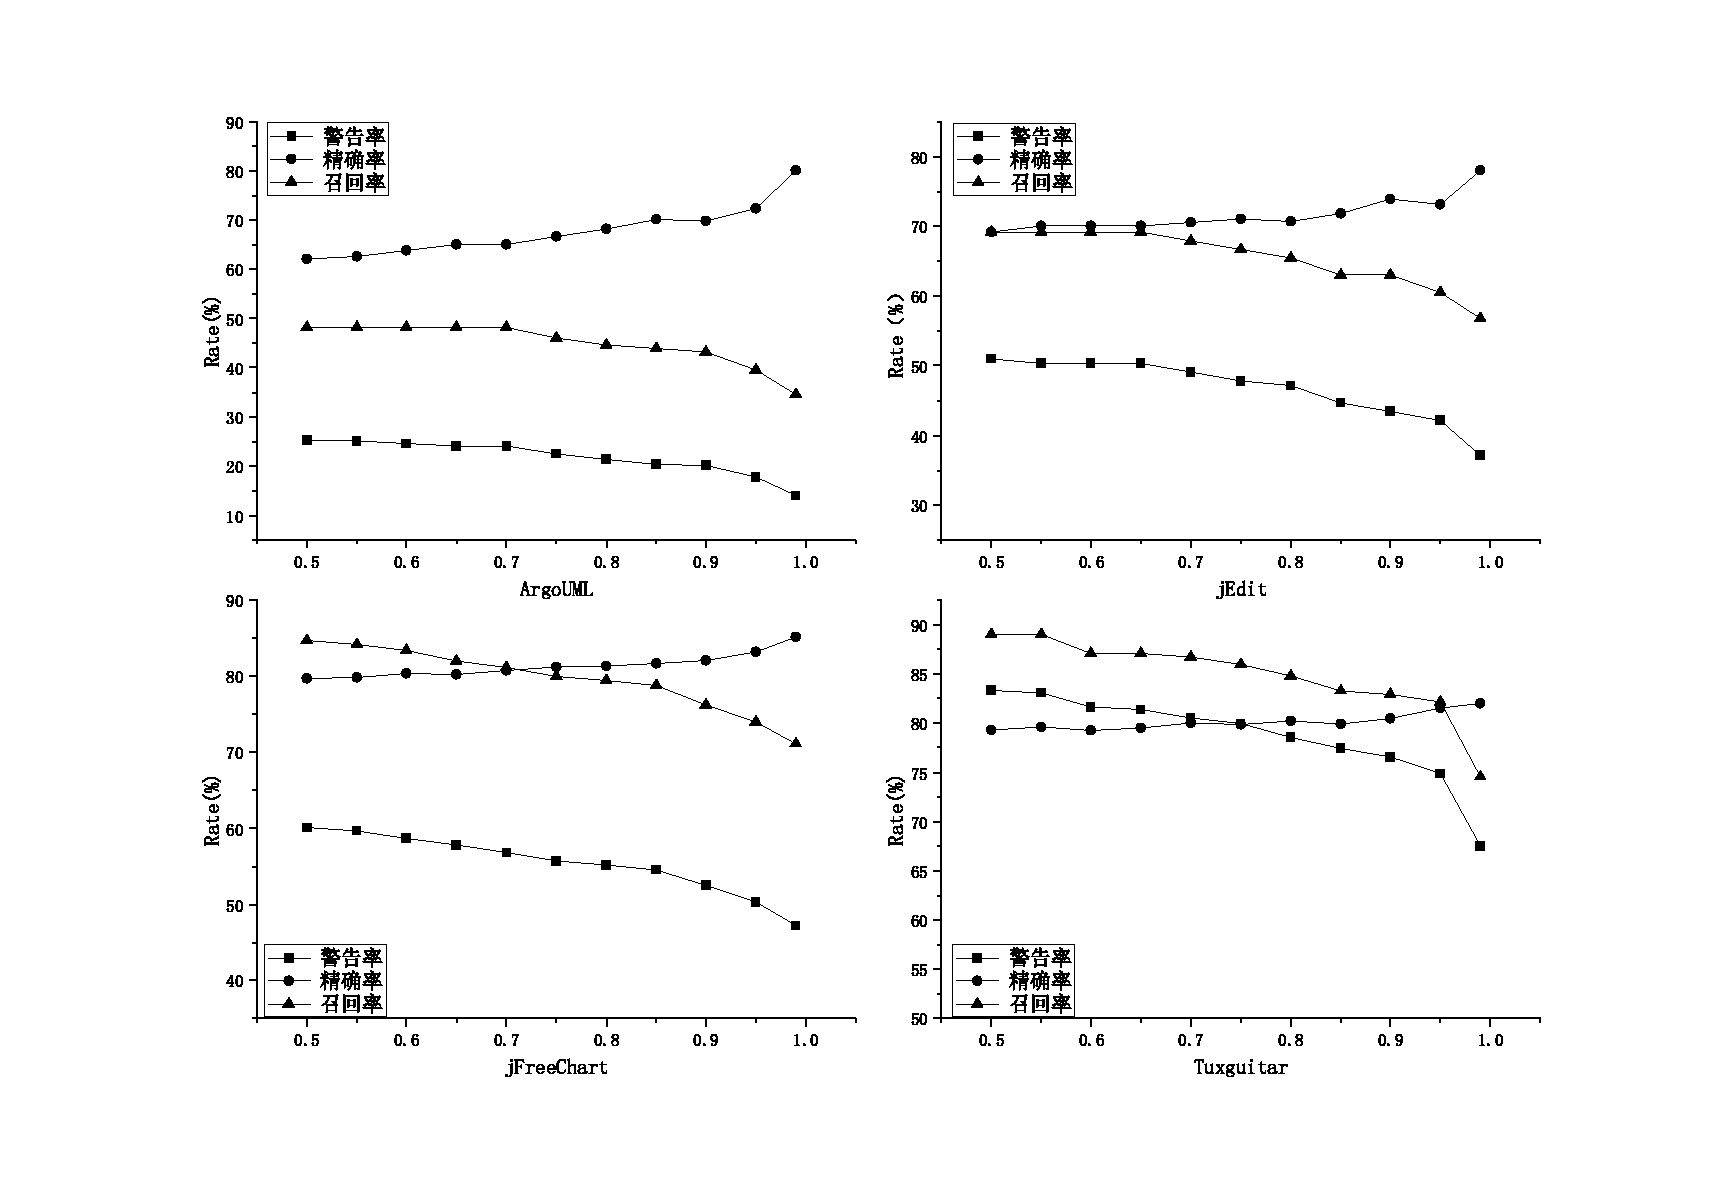
\includegraphics[width = 1.0\textwidth]{bayesgraph/changingallmeeting.pdf}
\bicaption[changingallmeeting]{}{全属性组需要维护的实验效果}
{Fig.$\!$}{The effectiveness for all attribute sets of clone consistency}
\vspace{-1em}
\end{figure}

由图中可以看出,所构建的模型在预测jFreeChart和Tuxguitar系统的一致性需求时,预测效果非常有效,其中预测的精确率和召回率在80\%左右。同时,jEdit系统的预测效果虽然不如上面两个系统好,但是也相当不错,精确率和召回率在70\%左右。原因可能是因为jEdit系统的克隆变化实例规模较小,没有对模型实现较好的训练,但这需要进一步验证研究。尽管ArgoUML的预测效果不如其它系统的预测效果,但其精确率仍然可以达到65\%左右,且召回率在45\%左右。

对于四个实验系统,本章所构建的模型均具有有十分合理的警告率,警告率十分接近于满足一致性维护需求的克隆变化实例的比例(如表~\ref {changesta}~中所示)。虽然阈值的变化可以影响预测的精确率和召回率,但影响并不是十分的剧烈,对召回率的影响要比精确率的影响更大。这意味着本章所创建的模型可以提供相当准确的预测效果,但仍需进一步增强预测模型的召回能力。

因此,开发人员可以较为自信地依赖于本章的方法,对需要一致性维护的克隆变化实例进行预测。同时,还可以采用其它方法来避免那些需要一致性维护的克隆实例,例如采用第3章的方法在克隆创建时尽量避免避免那些可能会引发一致性维护的克隆实例。

%%%%全属性实验使用本章提取的全部属性组在四个实验系统上进行评估,实验结果如表~\ref{changeallmeeting}所示。
%%%%
%%%%所创建的模型在预测jFreeChart和Tuxguitar的一致性需求时,预测结果显示非常有效,其中预测的精确率和召回率在80\%左右。同时,jEdit系统的预测效果虽然不如上面两个系统好,但是也相当不错。原因可能是因为jEdit系统的克隆变化实例规模较小,没有对模型实现较好的预测,但这需要进一步研究。尽管ArgoUML的预测效果不如其它系统的预测效果,但其精确率仍然可以达到65\%左右,且召回率在45\%左右。最后,对于四个实验系统,本文所构建的模型均具有有十分合理的警告率,警告率十分接近于满足一致性维护需求的克隆变化实例的比例(如表~\ref {changesta}~中所示)。
%%%%
%%%%虽然阈值的变化可以影响预测的精确率和召回率,但影响并不是十分的剧烈,对召回率的影响要比精确率的影响更大。这意味着本文所创建的模型可以提供相当准确的预测效果,但仍需进一步增强预测模型的召回能力。因此,开发人员可以较为自信地依赖于本文的预测结果,但需要其它方法来避免那些预测为不需要一致性维护的错误实例,从而帮助提高模型的预测效果。一个简单简单有效的改进方法是在克隆创建时尽量避免避免那些可能会引发一致性维护的克隆实例,具体细节可参考本文第3章提出的克隆创建时克隆一致性预测方法。
%%%%
%%%%\begin{table}[htbp]
%%%%\bicaption[changeallmeeting]{}{需要维护的全属性组实验效果}
%%%%{Table$\!$}{The effectiveness for all attribute sets of clone consistency}
%%%%\vspace{0.5em}
%%%%\centering
%%%%\wuhao
%%%%\begin{tabular}{ccccc}
%%%%\toprule[1.5pt]
%%%%{实验系统}&{阈值}&{警告率(\%)}&{精确率(\%)}&{召回率(\%)}\\
%%%%\midrule[1pt]
%%%% \multirow{5}{*}{ArgoUML}
%%%%&0.9&	20.14&	69.77&	43.17\\
%%%%&0.8&	21.31&	68.13&	44.60\\
%%%%&0.7&	24.12&	65.05&	48.20\\
%%%%&0.6&	24.59&	63.81&	48.20\\
%%%%&0.5&	25.29&	62.04&	48.20\\
%%%%\hline
%%%%\multirow{5}{*}{jEdit}
%%%%&0.9&	43.40&	73.91&	62.96\\
%%%%&0.8&	47.17&	70.67&	65.43\\
%%%%&0.7&	49.06&	70.51&	67.90\\
%%%%&0.6&	50.31&	70.00&	69.14\\
%%%%&0.5&	50.94&	69.14&	69.14\\
%%%%\hline
%%%%\multirow{5}{*}{jFreeChart}
%%%%&0.9&	52.50&	82.05&	76.19\\
%%%%&0.8&	55.19&	81.36&	79.42\\
%%%%&0.7&	56.83&	80.71&	81.12\\
%%%%&0.6&	58.65&	80.33&	83.33\\
%%%%&0.5&	60.10&	79.68&	84.69\\
%%%%\hline
%%%%\multirow{5}{*}{Tuxguitar}
%%%%&0.9	&76.55&   80.44&	82.89\\
%%%%&0.8	&78.53&	80.22&	84.79\\
%%%%&0.7	&80.51&	80.00&	86.69\\
%%%%&0.6	&81.64&	79.24&	87.07\\
%%%%&0.5    &83.33&	79.32&	88.97\\
%%%%\bottomrule[1.5pt]
%%%%\end{tabular}
%%%%\end{table}

(2)属性组实验结果

本章提取的了三组属性表示克隆变化实例,从不同的角度描述了变化实例的特征。为评估不同的属性组对预测效果的作用,本节进行了属性组实验。图~\ref{changingsetmeeting}~中给出了属性组的评估实验结果。其中,使用“All”表示全属性实验结果,“Code”表示移除代码属性的实验结果,“Context”表示上下文属性的实验结果,“Evo”表示移除演化属性的实验结果。并使用“WR”表示警告率,“P”表示精确率,“R”表示召回率。

\begin{figure}[h]
\centering
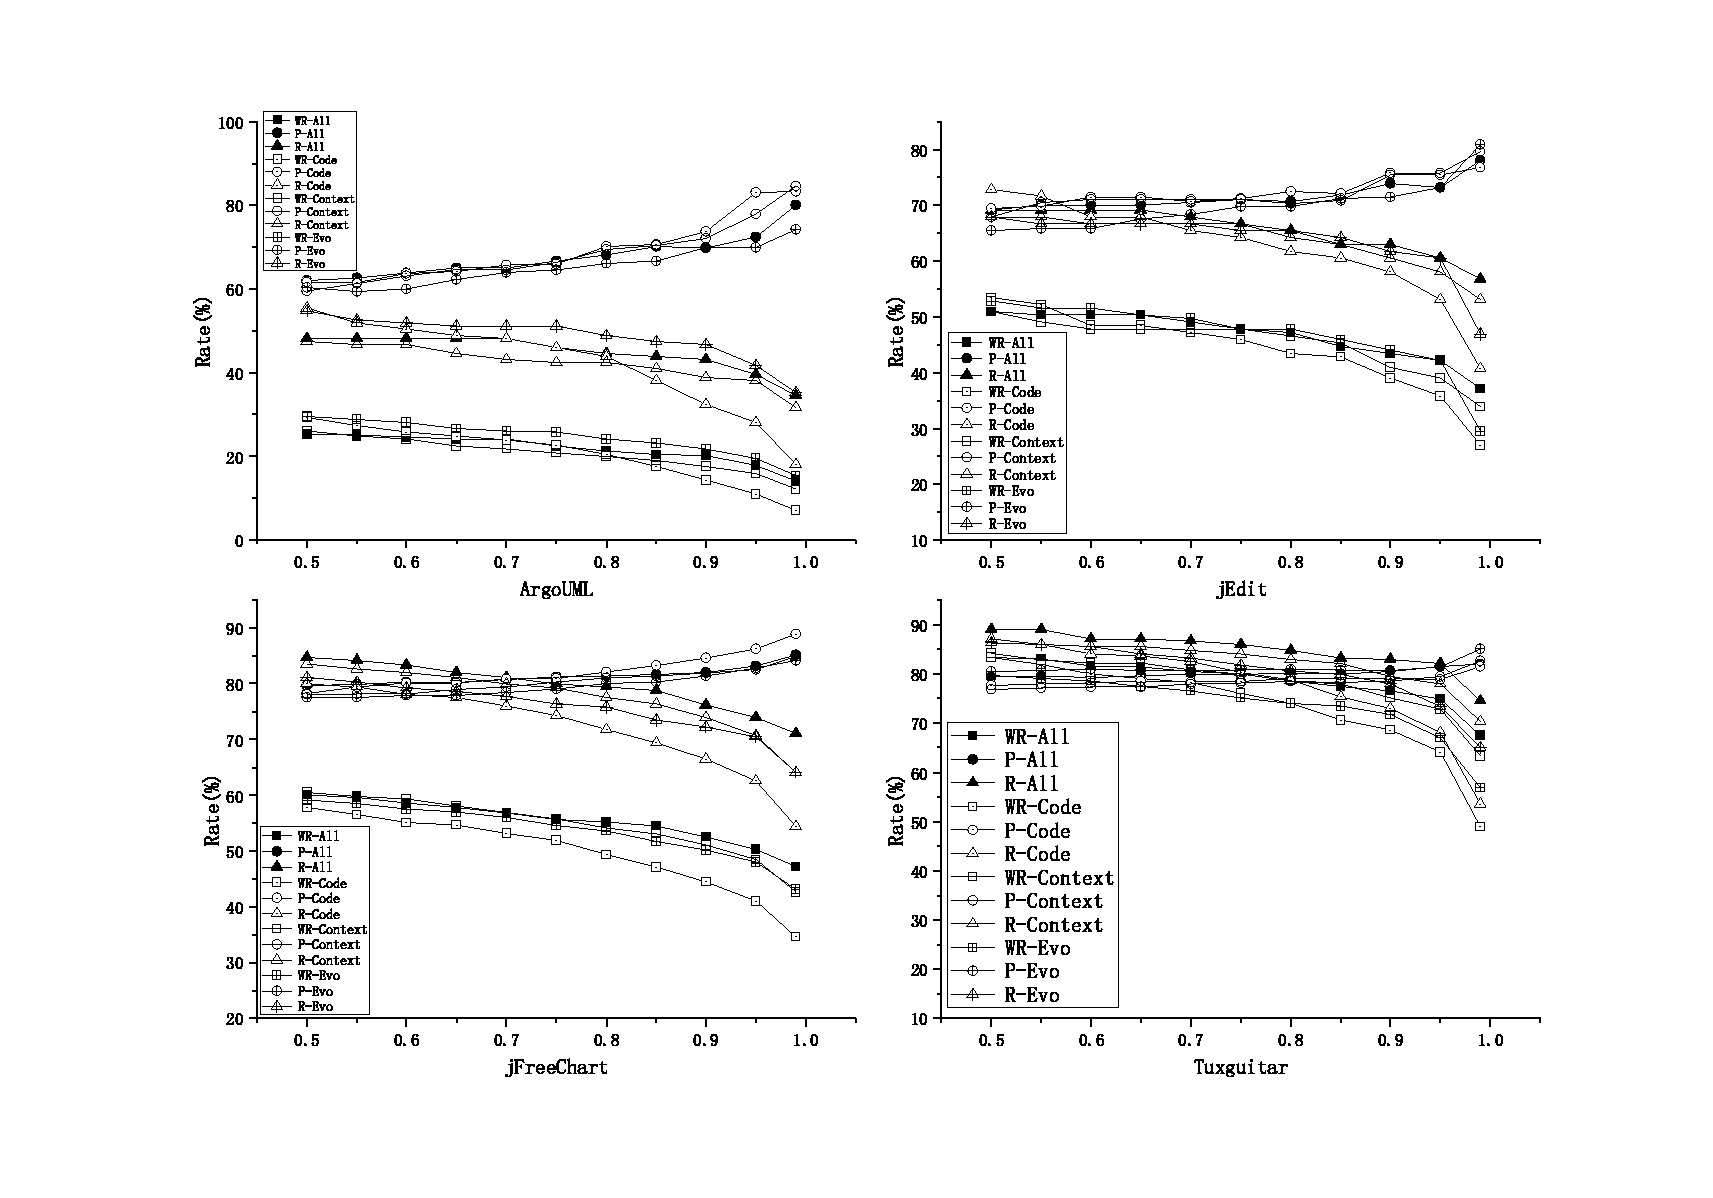
\includegraphics[width = 1.0\textwidth]{bayesgraph/changingsetmeeting.pdf}
\bicaption[changingsetmeeting]{}{需要维护的属性组实验效果}
{Fig.$\!$}{The effectiveness for attribute sets of clone consistency}
\vspace{-1em}
\end{figure}

从图中可以看出,属性组对预测结果的影响并无一致性结论。但是,代码属性和上下文属性与全属性组对比表明,这两组属性对预测的召回率有显著影响。但是,无演化组属性的实验结果表明其对实验结果的影响没有预想的那么大。尽管如此,这些属性组依然对预测效果有影响,但需要进一步的研究去寻找这种差异背后的真正原因。

此外,本章还对所选用的属性组进行了属性选择实验,使用WEKA提供的功能选取了最佳属性集。然而,通过比对全属性组的实验结果,发现发现全属性组实验结果要优于最佳属性组实验结果,所采用的属性具有积极的意义。虽然一些属性组可能对实验结果没有显着的影响,但是其也不具有消极的影响。本章建议在进行一致性预测时,需要保留全部属性组,因为在应用到其它系统是可能会起到积极的作用。
%%%表转图
%%%%%%本章提取的了三组属性表示克隆变化实例,从不同的角度描述了变化实例的特征。为评估不同的属性组对预测效果的作用,本节进行了属性组实验。表~\ref{changesetmeeting}~中给出了属性组的评估实验结果。其中,分别给出了使用全部属性和删除每一组属性后的实验结果,即“全部属性”、“无代码属性”、“无上下文属性”和“无演化属性”。
%%%%%%
%%%%%%从表中可以看出,属性组对预测结果的影响并无一致性结论。但是,代码属性和上下文属性与全属性组对比表明,这两组属性对预测的召回率有显著影响。但是,无演化组属性的实验结果表明其对实验结果的影响没有预想的那么大。尽管如此,这些属性组依然对预测效果有影响,但需要进一步的研究去寻找这种差异背后的真正原因。
%%%%%%
%%%%%%此外,本章还对所选用的属性组进行了属性选择实验,使用WEKA提供的功能选取了最佳属性集。然而,通过比对全属性组的实验结果,发现发现全属性组实验结果要优于最佳属性组实验结果,所采用的属性具有积极的意义。虽然一些属性组可能对实验结果没有显着的影响,但是其也不具有消极的影响。本章建议在进行一致性预测时,需要保留全部属性组,因为在应用到其它系统是可能会起到积极的作用。
%%%%%%
%%%%%表转图前
%%%%%%\begin{table} 
%%%%%%\renewcommand\arraystretch{0.65} 
%%%%%%\bicaption[changesetmeeting]{}{需要维护的属性组实验效果}
%%%%%%{Table$\!$}{The effectiveness for attribute set of clone consistency}
%%%%%%\vspace{0.5em}
%%%%%%\centering
%%%%%%\wuhao
%%%%%%\begin{tabular}{cccccccc}
%%%%%%\toprule[1.5pt]
%%%%%%{实验系统}&{实验组}&{指标}&{0.9}&{0.8}&{0.7}&{0.6}&{0.5}\\
%%%%%%\midrule[1pt]
%%%%%%\multirow{12}{*}{ArgoUML}
%%%%%%&~\multirow{3}{*}{全部属性(\%)}
%%%%%%& 警告率       & 20.14 & 21.31 & 24.12 & 24.59 & 25.29 \\
%%%%%%& & 精确率       & 69.77 & 68.13 & 65.05 & 63.81 & 62.04 \\
%%%%%%& & 召回率       & 43.17 & 44.60 & 48.20 & 48.20 & 48.20 \\
%%%%%%\cline{2-8}
%%%%%%&~\multirow{3}{*}{无代码属性    (\%)}
%%%%%%& 警告率       & 14.29 & 20.37 & 23.89 & 25.76 & 29.27 \\
%%%%%%&   & 精确率       & 73.77 & 70.11 & 65.69 & 63.64 & 61.60 \\
%%%%%% &  & 召回率       & 32.37 & 43.88 & 48.20 & 50.36 & 55.40 \\
%%%%%% \cline{2-8}
%%%%%%&~\multirow{3}{*}{无上下文属性   (\%)}
%%%%%%&       警告率       & 17.56 & 19.91 & 21.78 & 24.12 & 26.00 \\
%%%%%%& & 精确率       & 72.00 & 69.41 & 64.52 & 63.11 & 59.46 \\
%%%%%%&             & 召回率       & 38.85 & 42.45 & 43.17 & 46.76 & 47.48 \\
%%%%%%\cline{2-8}
%%%%%%&~\multirow{3}{*}{无演化属性(\%)}
%%%%%%&    警告率       & 21.78 & 24.12 & 26.00 & 28.10 & 29.51 \\
%%%%%%&  & 精确率       & 69.89 & 66.02 & 63.96 & 60.00 & 60.32 \\
%%%%%% &             & 召回率       & 46.76 & 48.92 & 51.08 & 51.80 & 54.68 \\
%%%%%% \hline
%%%%%%\multirow{12}{*}{jEdit     }
%%%%%%&~\multirow{3}{*}{全部属性(\%)}
%%%%%%&     警告率       & 43.40 & 47.17 & 49.06 & 50.31 & 50.94 \\
%%%%%% &   & 精确率       & 73.91 & 70.67 & 70.51 & 70.00 & 69.14 \\
%%%%%%&             & 召回率       & 62.96 & 65.43 & 67.90 & 69.14 & 69.14 \\
%%%%%%\cline{2-8}
%%%%%%&~\multirow{3}{*}{无代码属性 (\%)}
%%%%%%&   警告率       & 38.99 & 43.40 & 47.17 & 48.43 & 53.46 \\
%%%%%%&  & 精确率       & 75.81 & 72.46 & 70.67 & 71.43 & 69.41 \\
%%%%%%&             & 召回率       & 58.02 & 61.73 & 65.43 & 67.90 & 72.84 \\
%%%%%%\cline{2-8}
%%%%%%&~\multirow{3}{*}{无上下文属性   (\%)}
%%%%%%&    警告率       & 40.88 & 46.54 & 47.80 & 47.80 & 50.94 \\
%%%%%%&  & 精确率       & 75.38 & 70.27 & 71.05 & 71.05 & 67.90 \\
%%%%%%&   & 召回率       & 60.49 & 64.20 & 66.67 & 66.67 & 67.90 \\
%%%%%%\cline{2-8}
%%%%%%&~\multirow{3}{*}{无演化属性(\%)}
%%%%%%&   警告率       & 44.03 & 47.80 & 49.69 & 51.57 & 52.83 \\
%%%%%% &  & 精确率       & 71.43 & 69.74 & 68.35 & 65.85 & 65.48 \\
%%%%%%&             & 召回率       & 61.73 & 65.43 & 66.67 & 66.67 & 67.90 \\
%%%%%% \hline
%%%%%%\multirow{12}{*}{jFreeChart  }
%%%%%%&~\multirow{3}{*}{全部属性(\%)}
%%%%%%&    警告率       & 52.50 & 55.19 & 56.83 & 58.65 & 60.10 \\
%%%%%% &   & 精确率       & 82.05 & 81.36 & 80.71 & 80.33 & 79.68 \\
%%%%%%&             & 召回率       & 76.19 & 79.42 & 81.12 & 83.33 & 84.69 \\
%%%%%% \cline{2-8}
%%%%%%&~\multirow{3}{*}{无代码属性(\%)}
%%%%%%&   警告率       & 44.42 & 49.42 & 53.17 & 55.10 & 57.79 \\
%%%%%% &       & 精确率       & 84.63 & 82.10 & 80.83 & 80.10 & 78.20 \\
%%%%%%&             & 召回率       & 66.50 & 71.77 & 76.02 & 78.06 & 79.93 \\
%%%%%% \cline{2-8}
%%%%%% &~\multirow{3}{*}{无上下文属性(\%)}         
%%%%%% &   警告率       & 51.06 & 54.13 & 56.92 & 59.33 & 60.48 \\
%%%%%%&    & 精确率       & 81.92 & 80.99 & 79.39 & 78.12 & 78.06 \\
%%%%%% &             & 召回率       & 73.98 & 77.55 & 79.93 & 81.97 & 83.50 \\
%%%%%% \cline{2-8}
%%%%%%&~\multirow{3}{*}{无演化属性(\%)}    
%%%%%%&    警告率       & 50.19 & 53.56 & 56.06 & 57.50 & 59.13 \\
%%%%%%&  & 精确率       & 81.42 & 80.07 & 78.39 & 77.93 & 77.56 \\
%%%%%%&             & 召回率       & 72.28 & 75.85 & 77.72 & 79.25 & 81.12 \\
%%%%%%\hline
%%%%%%\multirow{12}{*}{Tuxguitar  }
%%%%%%&~\multirow{3}{*}{全部属性(\%)}
%%%%%% &   警告率       & 76.55 & 78.53 & 80.51 & 81.64 & 83.33 \\
%%%%%%&     & 精确率       & 80.44 & 80.22 & 80.00 & 79.24 & 79.32 \\
%%%%%% &             & 召回率       & 82.89 & 84.79 & 86.69 & 87.07 & 88.97 \\
%%%%%%\cline{2-8}
%%%%%%  &~\multirow{3}{*}{无代码属性(\%)}
%%%%%%& 警告率       & 68.64 & 74.01 & 78.25 & 79.94 & 83.33 \\
%%%%%% & & 精确率       & 79.01 & 79.01 & 78.34 & 78.09 & 77.63 \\
%%%%%% &             & 召回率       & 73.00 & 78.71 & 82.51 & 84.03 & 87.07 \\
%%%%%%  \cline{2-8}
%%%%%%&~\multirow{3}{*}{无上下文属性(\%)}
%%%%%%&    警告率       & 75.14 & 78.53 & 80.79 & 82.20 & 84.18 \\
%%%%%%&    & 精确率       & 78.57 & 78.42 & 77.97 & 77.32 & 76.85 \\
%%%%%% &             & 召回率       & 79.47 & 82.89 & 84.79 & 85.55 & 87.07 \\
%%%%%%\cline{2-8}
%%%%%%&~\multirow{3}{*}{无演化属性 (\%)}
%%%%%%&    警告率       & 71.75 & 74.01 & 76.55 & 78.53 & 79.66 \\
%%%%%% & & 精确率       & 80.71 & 80.92 & 80.81 & 80.94 & 80.50 \\
%%%%%%  &             & 召回率       & 77.95 & 80.61 & 83.27 & 85.55 & 86.31\\
%%%%%%\bottomrule[1.5pt]
%%%%%%\end{tabular}
%%%%%%\end{table}

%%%%以下是未经转置的全部实验结果
%%%%\begin{sidewaystable} 
%%%%\bicaption[changesetmeeting]{}{在四个实验系统上属性组实验效果}
%%%%{Table$\!$}{The effectiveness for attribute set on four projects}
%%%%\vspace{0.5em}
%%%%\centering
%%%%\wuhao
%%%%\begin{tabular}{cccccccccccccc}
%%%%\toprule[1.5pt]
%%%%\multirow{2}{*}{实验系统}&\multirow{2}{*}{阈值}&\multicolumn{3}{c}{全部属性(\%)}&\multicolumn{3}{c}{无代码属性(\%)}&\multicolumn{3}{c}{无上下文属性(\%)}&\multicolumn{3}{c}{无演化属性(\%)}\\
%%%%\cline{3-14}
%%%%&&{警告率}&{精确率}&{召回率}&{警告率}&{精确率}&{召回率}&{警告率}&{精确率}&{召回率}&{警告率}&{精确率}&{召回率}\\
%%%%\midrule[1pt]
%%%%\multirow{5}{*}{ArgoUML}
%%%%&0.9&20.14&	69.77&	43.17&14.29&	73.77&	32.37&17.56&	72.00&	38.85&21.78&	69.89&	46.76\\
%%%%&0.8&	21.31&	68.13&	44.60&	20.37&	70.11&	43.88&	19.91&	69.41&	42.45&	24.12&	66.02&	48.92\\
%%%%&0.7&	24.12&	65.05&	48.20&	23.89&	65.69&	48.20&	21.78&	64.52&	43.17&	26.00&	63.96&	51.08\\
%%%%&0.6&	24.59&	63.81&	48.20&	25.76&	63.64&	50.36&	24.12&	63.11&	46.76&	28.10&	60.00&	51.80\\
%%%%&0.5&	25.29&	62.04&	48.20&	29.27&	61.60&	55.40&	26.00&	59.46&	47.48&	29.51&	60.32&	54.68\\
%%%%\hline
%%%%\multirow{5}{*}{jEdit}
%%%%&0.9&	43.40&	73.91&	62.96&	38.99&	75.81&	58.02&	40.88&	75.38&	60.49&	44.03&	71.43&	61.73\\
%%%%&0.8&	47.17&	70.67&	65.43&	43.40&	72.46&	61.73&	46.54&	70.27&	64.20&	47.80&	69.74&	65.43\\
%%%%&0.7&	49.06&	70.51&	67.90&	47.17&	70.67&	65.43&	47.80&	71.05&	66.67&	49.69&	68.35&	66.67\\
%%%%&0.6&	50.31&	70.00&	69.14&	48.43&	71.43&	67.90&	47.80&	71.05&	66.67&	51.57&	65.85&	66.67\\
%%%%&0.5&	50.94&	69.14&	69.14&	53.46&	69.41&	72.84&	50.94&	67.90&	67.90&	52.83&	65.48&	67.90\\
%%%%\hline
%%%%\multirow{5}{*}{jFreeChart}
%%%%&0.9&	52.50&	82.05&	76.19&	44.42&	84.63&	66.50&	51.06&	81.92&	73.98&	50.19&	81.42&	72.28\\
%%%%&0.8&	55.19&	81.36&	79.42&	49.42&	82.10&	71.77&	54.13&	80.99&	77.55&	53.56&	80.07&	75.85\\
%%%%&0.7&	56.83&	80.71&	81.12&	53.17&	80.83&	76.02&	56.92&	79.39&	79.93&	56.06&	78.39&	77.72\\
%%%%&0.6&	58.65&	80.33&	83.33&	55.10&	80.10&	78.06&	59.33&	78.12&	81.97&	57.50&	77.93&	79.25\\
%%%%&0.5&	60.10&	79.68&	84.69&	57.79&	78.20&	79.93&	60.48&	78.06&	83.50&	59.13&	77.56&	81.12\\
%%%%\hline
%%%%\multirow{5}{*}{Tuxguitar}
%%%%&0.9&	76.55&	80.44&	82.89&	68.64&	79.01&	73.00&	75.14&	78.57&	79.47&	71.75&	80.71&	77.95\\
%%%%&0.8&	78.53&	80.22&	84.79&	74.01&	79.01&	78.71&	78.53&	78.42&	82.89&	74.01&	80.92&	80.61\\
%%%%&0.7&	80.51&	80.00&	86.69&	78.25&	78.34&	82.51&	80.79&	77.97&	84.79&	76.55&	80.81&	83.27\\
%%%%&0.6&	81.64&	79.24&	87.07&	79.94&	78.09&	84.03&	82.20&	77.32&	85.55&	78.53&	80.94&	85.55\\
%%%%&0.5&	83.33&	79.32&	88.97&	83.33&	77.63&	87.07&	84.18&	76.85&	87.07&	79.66&	80.50&      86.31\\
%%%%\bottomrule[1.5pt]
%%%%\end{tabular}
%%%%\end{sidewaystable}

\BiSubsubsection{一致性维护自由实验}
{The Experiment for Clone Changing Consistency-Free }

本节实验对不需要一致性维护的克隆变化实例进行预测评估。关注不需要一致性维护的克隆变化实例,让程序开发人员可以更加自由的修改克隆代码,而不需要考虑克隆变化所引发的一致性维护问题。此实验使用三个度量评估预测效果,分别为:推荐率、精确率和召回率。其中,推荐率指的是所推荐的不需要一致性维护的克隆变化实例与所有实例的比例,即预测为不需要一致性维护的克隆变化实例与系统中全部变化实例的比值。

%%%\begin{itemize}
%%%\item 
%%%推荐率(Recommendation Rate):
%%%指的是所推荐的不需要一致性维护的克隆变化实例与所有实例的比例,即预测为不需要一致性维护的克隆变化实例与系统中全部变化实例的比值。
%%%\item 
%%%精确率(Precision):
%%%指所预测的不需要一致性维护克隆变化实例的精确率,即在预测为不需要一致性维护的克隆变化实例中,正确预测的实例与所预测实例的比值。
%%%\item  
%%%召回率(Recall):
%%%指所推荐的不需要一致性维护的克隆变化实例的查全率,即预测为不需要一致性维护的变化实例,与系统中的不需要一致性维护的实例的比值。
%%%\end{itemize}

(1)全属性实验结果

全属性实验使用全部属性在四个实验系统上进行评估,实验结果如图~\ref{changingallfree}~所示。图中的横坐标表示阈值,设置阈值从0.01到0.50,图中的纵坐标为评价指标的数值大小。

\begin{figure}[h]
\centering
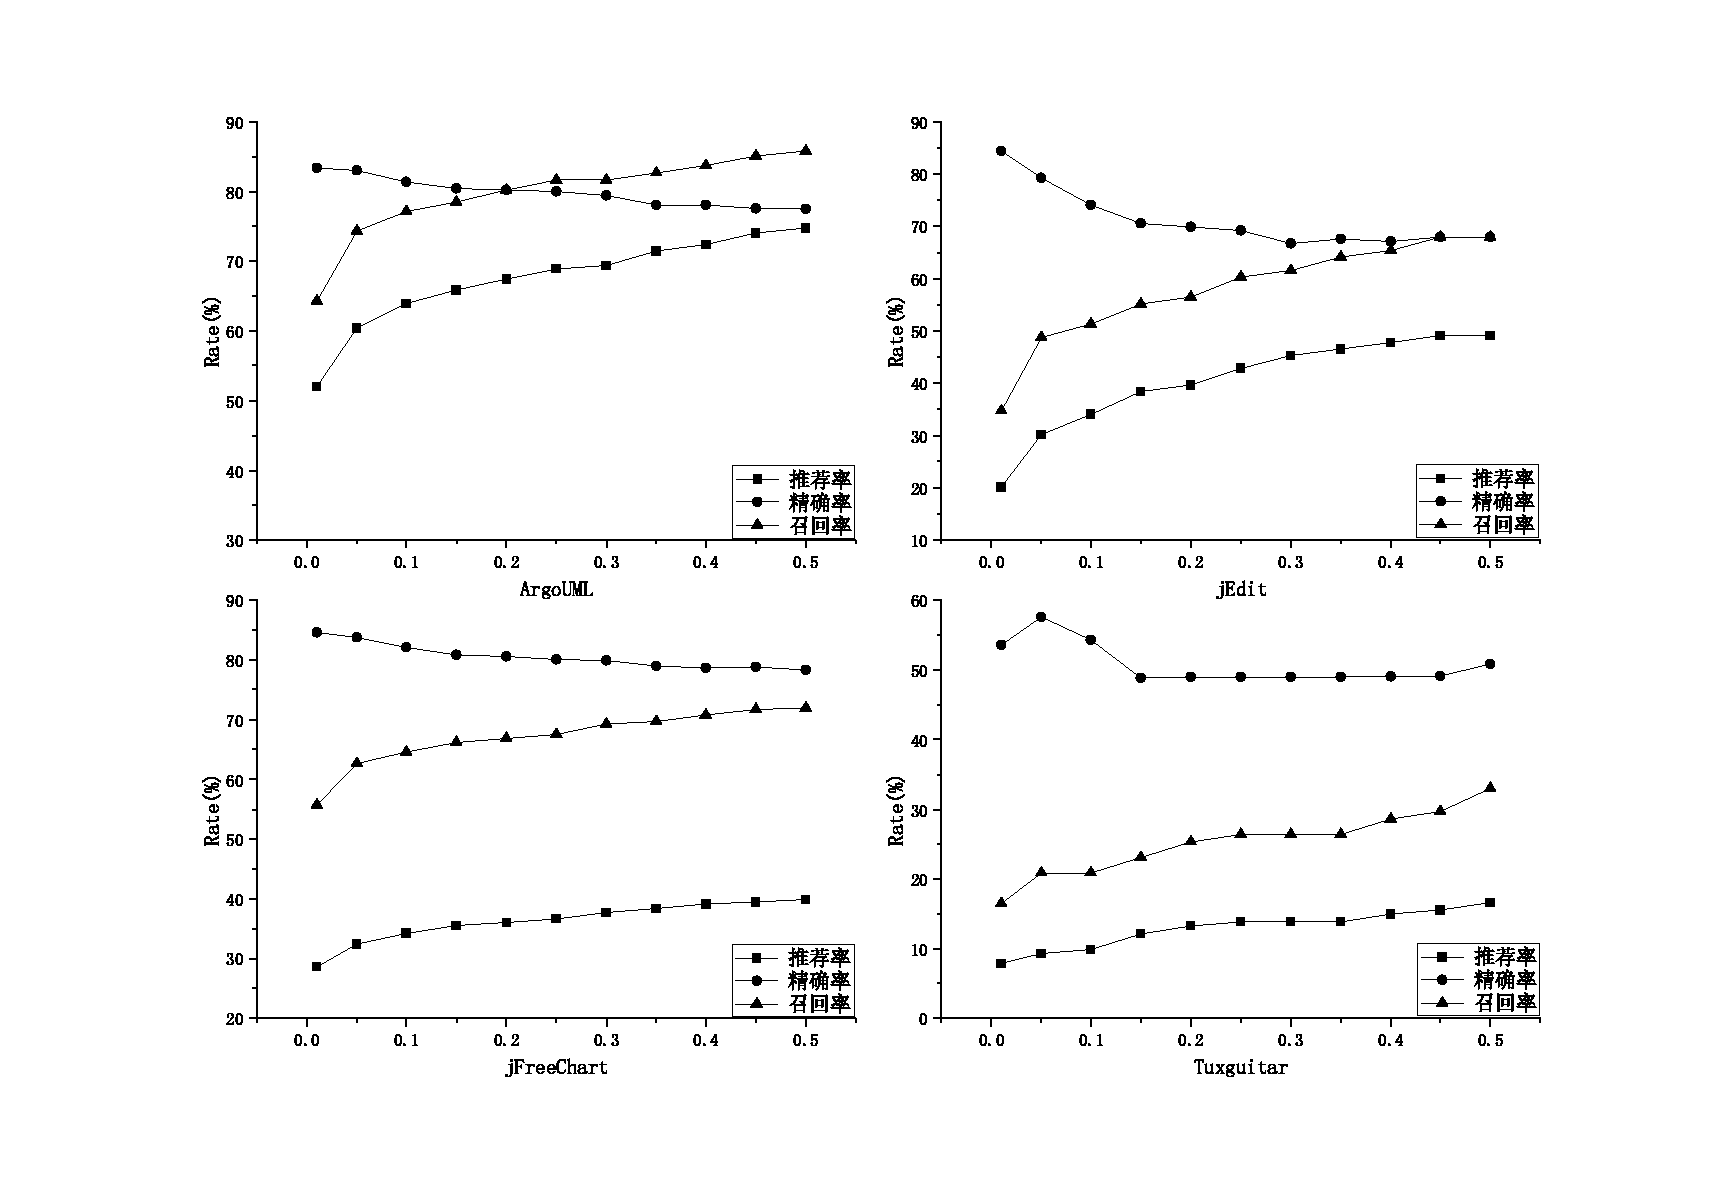
\includegraphics[width = 1.0\textwidth]{bayesgraph/changingallfree.pdf}
\bicaption[changingallfree]{}{全属性组维护自由实验效果}
{Fig.$\!$}{The effectiveness for all attributes of clone consistency free}
\vspace{-1em}
\end{figure}

由图中可以看出,本章方法在预测不需要一致性维护的克隆变化实例时,在四个系统上均取得了不错的预测效果。其中,在系统ArgoUML和 jFreeChart取得了较好的效果,精确率在80\%左右,并且召回率在70\%左右。在系统 jEdit的预测效果尽管没有上面两个系统的预测效果好,但也具有不错的预测效果。然而不幸的是,本章的方法在系统Tuxguitar上预测效果不够理想,精确率在50\%左右,召回率更低。可能是由于Tuxguitar的不满足一致性维护需求的克隆变化实例太少,没有对预测模型进行完全训练。

同时,由图~\ref{changingallfree}~和表~\ref{changesta}~ 可以看出,本章所构建的模型在四个系统上都具有十分合理的推荐率,推荐率和系统本身的不需要一致性维护的克隆变化的比例相差不大。与此同时,阈值会影响到预测的精确率和召回率,阈值对于召回率的影响要大于大于精确率的影响。这意味着本文所构建的模型可以较为稳定地进行一致性维护需求预测(精确率相差不大),但是系统的召回率仍需要进一步的提升。简而言之,本章的方法所构建的预测模型可以对不需要一致性维护的克隆变化实例提供一个相对稳定的预测,并且具有较好的精确率和召回率,软件开发人员可以据此对克隆变化实例进行有效的预测。

%%%全属性实验使用全部属性在四个实验系统上进行评估,实验结果如表~\ref{changeallfree}~所示。
%%%
%%%由表中可以看出,本文方法在预测不需要一致性维护的克隆变化实例时,在四个系统上均取得了不错的预测效果。其中,在系统ArgoUML和 jFreeChart取得了较好的效果,精确率在80\%左右,并且召回率在70\%左右。在系统 jEdit的预测效果尽管没有上面两个系统的预测效果好,但也具有不错的预测效果。然而不幸的是,本文的方法在系统Tuxguitar上预测效果不够理想,精确率在50\%左右,召回率更低。可能是由于Tuxguitar的不满足一致性维护需求的克隆变化实例太少,没有对预测模型训练完全,但是仍需进一步的研究确认。同时,本文所构建的模型在四个系统上都具有十分合理的推荐率,推荐率和系统本身的不需要一致性维护的克隆变化的比例相差不大(如表~\ref{changesta}~中所列)。
%%%
%%%不同的阈值会影响到精确率和召回率,但是阈值对于召回率的影响要大于大于精确率的影响。这意味着本文所构建的模型可以提高比较稳定的预测效果(精确率差不大),但系统的召回率仍需要进一步的提升。简而言之,本文的方法所构建的预测模型可以对不需要一致性维护的克隆变化实例提供一个相对稳定的预测,并且具有相当好的精确率和召回率,软件开发人员可以据此对克隆变化实例进行有效的预测。
%%%
%%%
%%%\begin{table}[htbp]
%%%\bicaption[changeallfree]{}{全属性组维护自由实验效果}
%%%{Table$\!$}{The effectiveness for all attribute of clone consistency free}
%%%\vspace{0.5em}
%%%\centering
%%%\wuhao
%%%\begin{tabular}{ccccc}
%%%\toprule[1.5pt]
%%%{系统}&{阈值}&{推荐率(\%)}&{精确率(\%)}&{召回率(\%)}\\
%%%\midrule[1pt]
%%%\multirow{5}{*}{ArgoUML}
%%%&0.01&	51.99&	83.33&	64.24\\
%%%&0.05&	60.42&	82.95&	74.31\\
%%%&0.1&	63.93&	81.32&	77.08\\
%%%&0.15&	65.81&	80.43&	78.47\\
%%%&0.2&	67.45&	80.21&	80.21\\
%%%\hline
%%%\multirow{5}{*}{jEdit}
%%%&0.01&	20.13&	84.38&	34.62\\
%%%&0.05&	30.19&	79.17&	48.72\\
%%%&0.1&	33.96&	74.07&	51.28\\
%%%&0.15&	38.36&	70.49&	55.13\\
%%%&0.2&	39.62&	69.84&	56.41\\
%%%\hline
%%%\multirow{5}{*}{jFreeChart}
%%%&0.01&	28.65&	84.56&	55.75\\
%%%&0.05&	32.50&	83.73&	62.61\\
%%%&0.1&	34.23&	82.02&	64.60\\
%%%&0.15&	35.58&	80.81&	66.15\\
%%%&0.2&	36.06&	80.53&	66.81\\
%%%\hline
%%%\multirow{5}{*}{Tuxguitar}
%%%&0.01&	7.91&	53.57&	16.48\\
%%%&0.05&	9.32&	57.58&	20.88\\
%%%&0.1&	9.89&	54.29&	20.88\\
%%%&0.15&	12.15&	48.84&	23.08\\
%%%&0.2&	13.28&	48.94&	25.27\\
%%%\bottomrule[1.5pt]
%%%\end{tabular}
%%%\end{table}

(2)属性组实验结果

针对不需要一致性维护的克隆变化实例,同样进行了属性组实验以评估不同的属性组对预测效果的影响。实验结果如图~\ref{changingsetfree}~所示。其中,使用“RR”表示推荐率,“P”表示精确率,“R”表示召回率。同时,使用“All”表示全属性实验结果,“Code”表示移除代码属性的实验结果,“Context”表示上下文属性的实验结果,“Evo”表示移除演化属性的实验结果。

\begin{figure}[h]
\centering
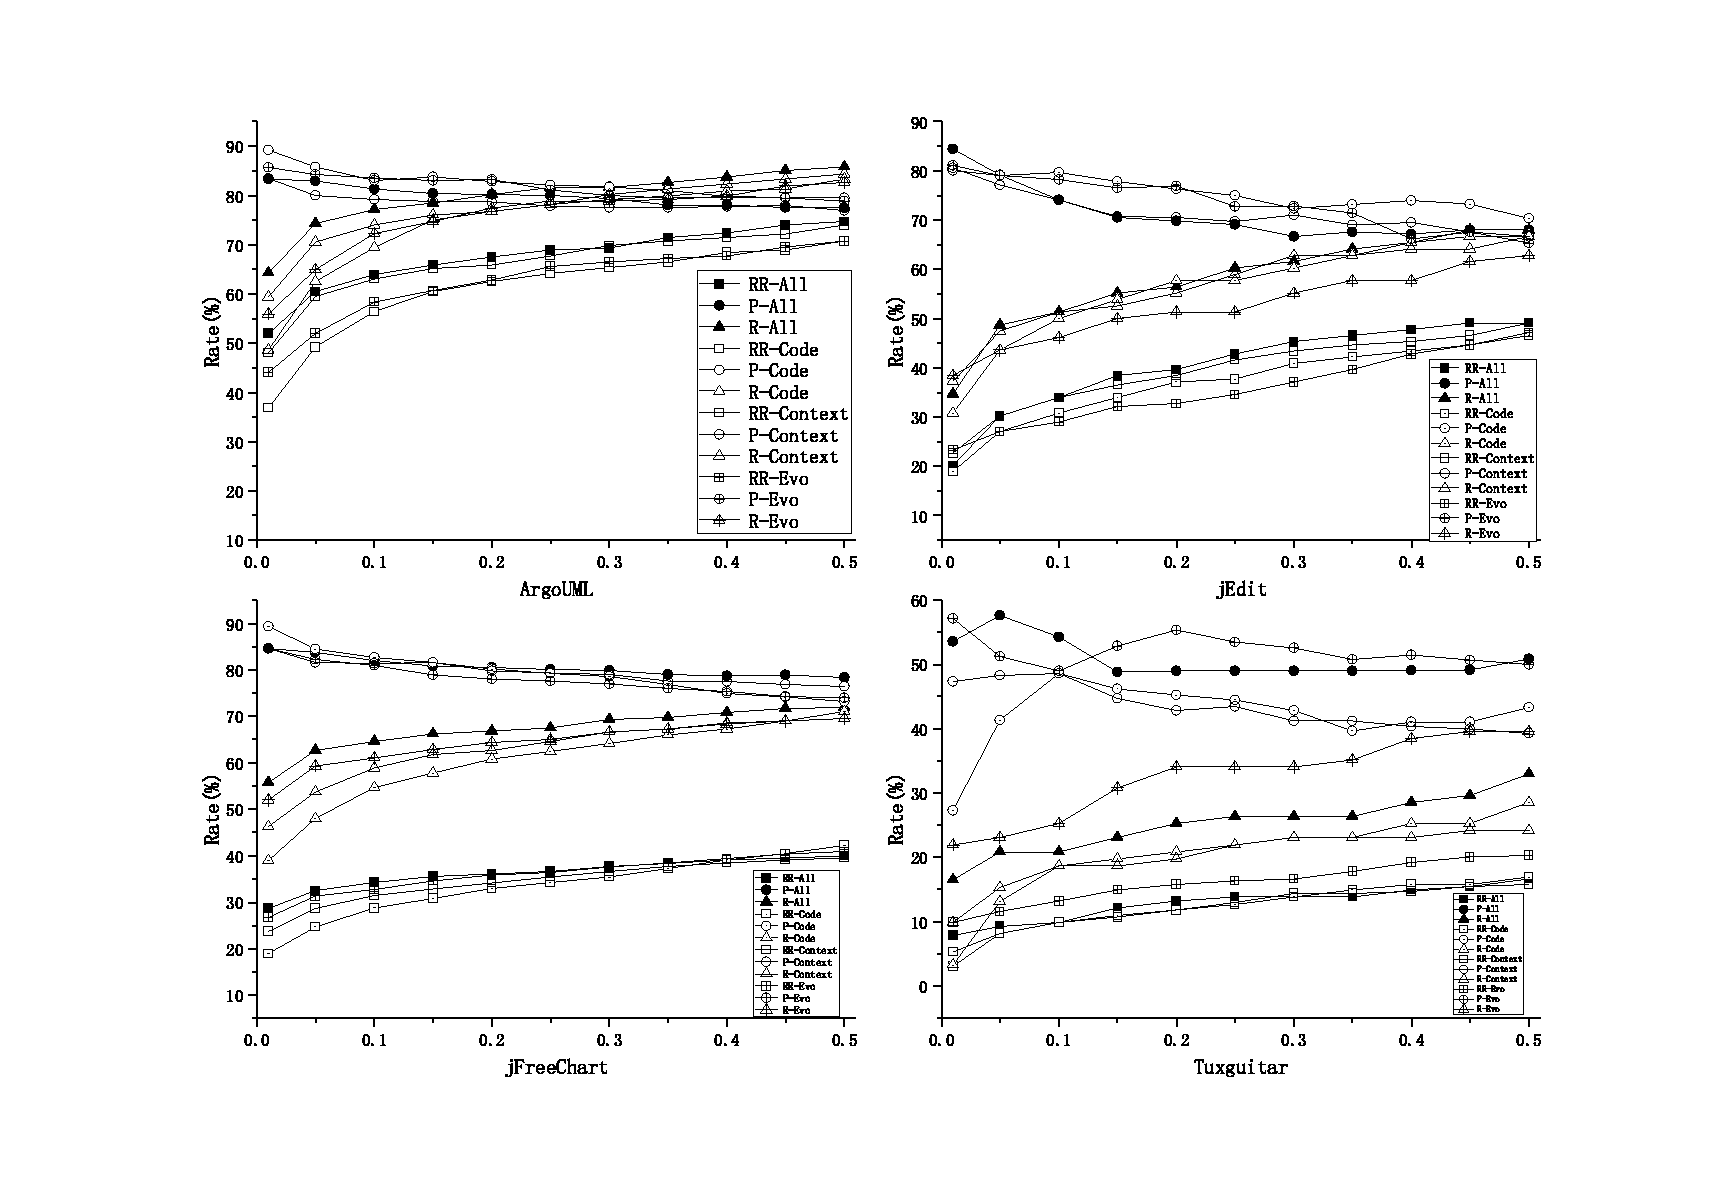
\includegraphics[width = 1.0\textwidth]{bayesgraph/changingsetfree.pdf}
\bicaption[changingsetfree]{}{属性组维护自由实验效果}
{Fig.$\!$}{The effectiveness for attribute set of clone consistency free}
\vspace{-1em}
\end{figure}

从图中可以看出,属性组对“一致性维护自由”实验的预测结果的影响并无一致性结论。但是,代码属性和上下文属性与全属性组对比表明,这两组属性对预测的召回率有显著影响。但是,无演化组属性的实验结果表明其对实验结果的影响没有预想的那么大。尽管如此,这些属性组依然对预测效果有积极的影响,但需要进一步的研究去寻找这种差异背后的真正原因。

此外,本章还对所选用的属性组进行了属性选择实验,使用WEKA提供的功能选取了最佳属性集。然而,通过比对全属性组的实验结果,发现发现全属性组实验结果要好于最佳属性子集的实验结果,因此,所采用的属性具有积极的意义。虽然一些属性组可能对实验结果没有显着的影响,但是其也不具有消极的影响。

尽管一些属性组可能对实验结果没有极为重要的贡献,但是属性组同样也没有产生消极的影响。因此,本章建议将所有属性保留在构建预测模型中,因为某些属性可能对一些未经实验验证的系统具有重要且积极的影响。

%%%同样,对不需要一致性维护的克隆变化实例,本章同样进行了属性组实验,以评估不同的属性组对预测效果的影响。实验结果如表~\ref{changesetfree}~所示,其中,分别给出了使用全部属性和删除每一组属性后的实验结果,即“全部属性”、“无代码属性”、“无上下文属性”和“无演化属性”。
%%%
%%%从表中可以看出,属性组对“一致性维护自由”实验的预测结果的影响并无一致性结论。但是,代码属性和上下文属性与全属性组对比表明,这两组属性对预测的召回率有显著影响。但是,无演化组属性的实验结果表明其对实验结果的影响没有预想的那么大。尽管如此,这些属性组依然对预测效果有影响,但需要进一步的研究去寻找这种差异背后的真正原因。
%%%
%%%此外,本文还对所选用的属性组进行了属性选择实验,使用WEKA提供的功能选取了最佳属性集。然而,通过比对全属性组的实验结果,发现发现全属性组实验结果要好于最佳属性子集的实验结果,因此,所采用的属性具有积极的意义。虽然一些属性组可能对实验结果没有显着的影响,但是其也不具有消极的影响。
%%%
%%%尽管一些属性组可能对实验结果没有极为重要的贡献,但是属性组同样也没有产生消极的影响。因此,本文建议将所有属性保留在构建预测模型中,因为某些属性可能对一些未经实验验证的系统具有重要且积极的影响。
%%%
%%%表转图前
%%%\begin{table} 
%%%\renewcommand\arraystretch{0.65} 
%%%\bicaption[changesetfree]{}{属性组维护自由实验效果}
%%%{Table$\!$}{The effectiveness for attribute set of clone consistency free}
%%%\vspace{0.5em}
%%%\centering
%%%\wuhao
%%%\begin{tabular}{cccccccc}
%%%\toprule[1.5pt]
%%%{实验系统}&{实验组}&{指标}&{0.01}&{0.05}&{0.1}&{0.15}&{0.2}\\
%%%\midrule[1pt]
%%%\multirow{12}{*}{ArgoUML}
%%%&~\multirow{3}{*}{全部属性(\%) }
%%%& 推荐率 & 51.99 & 60.42 & 63.93 & 65.81 & 67.45 \\
%%%&& 精确率 & 83.33 & 82.95 & 81.32 & 80.43 & 80.21 \\
%%%& & 召回率 & 64.24 & 74.31 & 77.08 & 78.47 & 80.21 \\
%%%\cline{2-8}
%%%&~\multirow{3}{*}{无代码属性(\%)}    
%%%& 推荐率 & 36.77 & 49.18 & 56.67 & 60.42 & 62.53 \\
%%%& & 精确率 & 89.17 & 85.71 & 83.06 & 83.72 & 82.77 \\
%%%& &召回率 & 48.61 & 62.50 & 69.79 & 75.00 & 76.74 \\
%%%\cline{2-8}
%%%&~\multirow{3}{*}{无上下文属性(\%)}    
%%%& 推荐率 & 48.01 & 59.48 & 63.00 & 65.11 & 65.81 \\
%%%&& 精确率 & 83.41 & 79.92 & 79.18 & 78.78 & 78.65 \\
%%%&& 召回率 & 59.38 & 70.49 & 73.96 & 76.04 & 76.74 \\
%%%\cline{2-8}
%%%&~\multirow{3}{*}{无演化属性(\%)}    
%%%& 推荐率 & 44.03 & 51.99 & 58.31 & 60.66 & 62.76 \\
%%%&  & 精确率 & 85.64 & 84.23 & 83.53 & 83.01 & 83.21 \\
%%%& & 召回率 & 55.90 & 64.93 & 72.22 & 74.65 & 77.43 \\
%%%\hline
%%%\multirow{12}{*}{jEdit}
%%%&~\multirow{3}{*}{全部属性(\%) }
%%%& 推荐率 & 20.13 & 30.19 & 33.96 & 38.36 & 39.62 \\
%%%&  &精确率 & 84.38 & 79.17 & 74.07 & 70.49 & 69.84 \\
%%%& & 召回率 & 34.62 & 48.72 & 51.28 & 55.13 & 56.41 \\
%%%\cline{2-8}
%%%&~\multirow{3}{*}{无代码属性(\%)}    
%%%& 推荐率 & 18.87 & 27.04 & 30.82 & 33.96 & 37.11 \\
%%%&  &精确率 & 80.00 & 79.07 & 79.59 & 77.78 & 76.27 \\
%%%&  &召回率 & 30.77 & 43.59 & 50.00 & 53.85 & 57.69 \\
%%%\cline{2-8}
%%%&~\multirow{3}{*}{无上下文属性(\%)}    
%%%& 推荐率 & 22.64 & 30.19 & 33.96 & 36.48 & 38.36 \\
%%%&  &精确率 & 80.56 & 77.08 & 74.07 & 70.69 & 70.49 \\
%%%&  &召回率 & 37.18 & 47.44 & 51.28 & 52.56 & 55.13 \\
%%%\cline{2-8}
%%%&~\multirow{3}{*}{无演化属性(\%)}    
%%%& 推荐率 & 23.27 & 27.04 & 28.93 & 32.08 & 32.70 \\
%%%&  &精确率 & 81.08 & 79.07 & 78.26 & 76.47 & 76.92 \\
%%%&  &召回率 & 38.46 & 43.59 & 46.15 & 50.00 & 51.28 \\
%%%\hline
%%%\multirow{12}{*}{jFreeChart}
%%%&~\multirow{3}{*}{全部属性(\%) }
%%%& 推荐率 & 28.65 & 32.50 & 34.23 & 35.58 & 36.06 \\
%%%&  &精确率 & 84.56 & 83.73 & 82.02 & 80.81 & 80.53 \\
%%%&  &召回率 & 55.75 & 62.61 & 64.60 & 66.15 & 66.81 \\
%%%\cline{2-8}
%%%&~\multirow{3}{*}{无代码属性(\%)}    
%%% & 推荐率 & 18.94 & 24.71 & 28.75 & 30.77 & 32.98 \\
%%%&  &精确率 & 89.34 & 84.44 & 82.61 & 81.56 & 80.17 \\
%%%&  &召回率 & 38.94 & 48.01 & 54.65 & 57.74 & 60.84 \\
%%%\cline{2-8}
%%%&~\multirow{3}{*}{无上下文属性(\%)}    
%%%& 推荐率 & 23.75 & 28.65 & 31.44 & 32.88 & 34.13 \\
%%%&  &精确率 & 84.62 & 81.54 & 81.35 & 81.58 & 79.72 \\
%%%&  &召回率 & 46.24 & 53.76 & 58.85 & 61.73 & 62.61 \\
%%%\cline{2-8}
%%%&~\multirow{3}{*}{无演化属性(\%)}    
%%%& 推荐率 & 26.73 & 31.35 & 32.79 & 34.62 & 35.87 \\
%%%&  &精确率 & 84.53 & 82.21 & 80.94 & 78.89 & 78.02 \\
%%%&  &召回率 & 51.99 & 59.29 & 61.06 & 62.83 & 64.38 \\
%%%\hline
%%%\multirow{12}{*}{Tuxguitar}
%%%&~\multirow{3}{*}{全部属性(\%) }
%%%& 推荐率 & 7.91  & 9.32  & 9.89  & 12.15 & 13.28 \\
%%%&  &精确率 & 53.57 & 57.58 & 54.29 & 48.84 & 48.94 \\
%%%&  &召回率 & 16.48 & 20.88 & 20.88 & 23.08 & 25.27 \\
%%%\cline{2-8}
%%%&~\multirow{3}{*}{无代码属性(\%)}    
%%%& 推荐率 & 3.11  & 8.19  & 9.89  & 11.02 & 11.86 \\
%%%&  &精确率 & 27.27 & 41.38 & 48.57 & 46.15 & 45.24 \\
%%%&  &召回率 & 3.30  & 13.19 & 18.68 & 19.78 & 20.88 \\
%%%\cline{2-8}
%%%&~\multirow{3}{*}{无上下文属性 (\%)}    
%%% & 推荐率 & 5.37  & 8.19  & 9.89  & 10.73 & 11.86 \\
%%%&  &精确率 & 47.37 & 48.28 & 48.57 & 44.74 & 42.86 \\
%%%&  &召回率 & 9.89  & 15.38 & 18.68 & 18.68 & 19.78 \\
%%%\cline{2-8}
%%%&~\multirow{3}{*}{无演化属性(\%)}    
%%%& 推荐率 & 9.89  & 11.58 & 13.28 & 14.97 & 15.82 \\
%%%&  &精确率 & 57.14 & 51.22 & 48.94 & 52.83 & 55.36 \\
%%%&  &召回率 & 21.98 & 23.08 & 25.27 & 30.77 & 34.07\\
%%%\bottomrule[1.5pt]
%%%\end{tabular}
%%%\end{table} 

%%%%以下是未经转置的全部实验结果
%%%\begin{sidewaystable} 
%%%\bicaption[changesetfree]{}{在四个实验系统上属性组实验效果}
%%%{Table$\!$}{The effectiveness for attribute set on four projects}
%%%\vspace{0.5em}
%%%\centering
%%%\wuhao
%%%\begin{tabular}{cccccccccccccc}
%%%\toprule[1.5pt]
%%%\multirow{2}{*}{实验系统}&\multirow{2}{*}{阈值}&\multicolumn{3}{c}{全部属性(\%)}&\multicolumn{3}{c}{无代码属性(\%)}&\multicolumn{3}{c}{无上下文属性(\%)}&\multicolumn{3}{c}{无演化属性(\%)}\\
%%%\cline{3-14}
%%%&&{警告率}&{精确率}&{召回率}&{警告率}&{精确率}&{召回率}&{警告率}&{精确率}&{召回率}&{警告率}&{精确率}&{召回率}\\
%%%\midrule[1pt]
%%%\multirow{5}{*}{ArgoUML}
%%%&0.01&	51.99&	83.33&	64.24&	36.77&	89.17&	48.61&	48.01&	83.41&	59.38&	44.03&	85.64&	55.90\\
%%%&0.05&	60.42&	82.95&	74.31&	49.18&	85.71&	62.50&	59.48&	79.92&	70.49&	51.99&	84.23&	64.93\\
%%%&0.1&	63.93&	81.32&	77.08&	56.67&	83.06&	69.79&	63.00&	79.18&	73.96&	58.31&	83.53&	72.22\\
%%%&0.15&	65.81&	80.43&	78.47&	60.42&	83.72&	75.00&	65.11&	78.78&	76.04&	60.66&	83.01&	74.65\\
%%%&0.2&	67.45&	80.21&	80.21&	62.53&	82.77&	76.74&	65.81&	78.65&	76.74&	62.76&	83.21&	77.43\\
%%%\hline
%%%\multirow{5}{*}{jEdit}
%%%&0.01&	20.13&	84.38&	34.62&	18.87&	80.00&	30.77&	22.64&	80.56&	37.18&	23.27&	81.08&	38.46\\
%%%&0.05&	30.19&	79.17&	48.72&	27.04&	79.07&	43.59&	30.19&	77.08&	47.44&	27.04&	79.07&	43.59\\
%%%&0.1&	33.96&	74.07&	51.28&	30.82&	79.59&	50.00&	33.96&	74.07&	51.28&	28.93&	78.26&	46.15\\
%%%&0.15&	38.36&	70.49&	55.13&	33.96&	77.78&	53.85&	36.48&	70.69&	52.56&	32.08&	76.47&	50.00\\
%%%&0.2&	39.62&	69.84&	56.41&	37.11&	76.27&	57.69&	38.36&	70.49&	55.13&	32.70&	76.92&	51.28\\
%%%\hline
%%%\multirow{5}{*}{jFreeChart}
%%%&0.01& 28.65&	84.56&	55.75&	18.94&	89.34&	38.94&	23.75&	84.62&	46.24&	26.73&	84.53&	51.99\\
%%%&0.05&	32.50&	83.73&	62.61&	24.71&	84.44&	48.01&	28.65&	81.54&	53.76&	31.35&	82.21&	59.29\\
%%%&0.1&	34.23&	82.02&	64.60&	28.75&	82.61&	54.65&	31.44&	81.35&	58.85&	32.79&	80.94&	61.06\\
%%%&0.15&	35.58&	80.81&	66.15&	30.77&	81.56&	57.74&	32.88&	81.58&	61.73&	34.62&	78.89&	62.83\\
%%%&0.2&	36.06&	80.53&	66.81&	32.98&	80.17&	60.84&	34.13&	79.72&	62.61&	35.87&	78.02&	64.38\\
%%%\hline
%%%\multirow{5}{*}{Tuxguitar}
%%%&0.01&	7.91&	53.57&	16.48&	3.11&	27.27&	3.30&	5.37&	47.37&	9.89&	9.89&	57.14&	21.98\\
%%%&0.05&	9.32&	57.58&	20.88&	8.19&	41.38&	13.19&	8.19&	48.28&	15.38&	11.58&	51.22&	23.08\\
%%%&0.1&	9.89&	54.29&	20.88&	9.89&	48.57&	18.68&	9.89&	48.57&	18.68&	13.28&	48.94&	25.27\\
%%%&0.15&	12.15&	48.84&	23.08&	11.02&	46.15&	19.78&	10.73&	44.74&	18.68&	14.97&	52.83&	30.77\\
%%%&0.2&	13.28&	48.94&	25.27&	11.86&	45.24&	20.88&	11.86&	42.86&	19.78&	15.82&	55.36&	34.07\\
%%%\bottomrule[1.5pt]
%%%\end{tabular}
%%%\end{sidewaystable} 

\BiSubsection{讨论}
{Discussion}

本节从不同的角度评估了本章所提出的克隆代码变化一致性维护需求预测,同时对需要和不需要一致性维护需求的克隆变化实例进行了预测,并从不同的角度评估了不同的机器学习方法的预测能力。

在有效性预测实验中,本章所提的方法是有效的。五种机器学习方法都可预测克隆变化的一致性维护需求,并具有相似的预测能力,预测结果具有合理的精确率、召回率和F值。更重要的是,不同机器学习模型的预测能力仅具有较小的差异,但支持向量机方法拥有相对最佳的预测效果。因此,建议优先推荐使用支持向量机方法预测克隆代码变化一致性维护需求。与此同时,所提取的属性组作为一个整体在不同机器学习方法中,同样起到了积极的作用,因此建议开发人员在预测时使用全部的属性组。

在使用模式实验中,全属性实验结果表明本章的模型在一致性维护需求和一致性维护自由的实验上均具有有效的预测能力。属性组实验表明每一个属性组在不同角度和程度上对预测模型的效果有着积极的作用。因此,鼓励开发人员使用全属性组进行克隆变化实例的一致性维护需求预测,从而将其适用到其它未验证的系统中,使之达到最佳的预测效果。

\BiSection{本章小结}
{Summary of this Chapter}

软件中存在的克隆代码的一致性变化,可能会引发克隆一致性违背缺陷。但是,现有的方法中尚无法在克隆代码变化时预测克隆代码的一致性变化,更无法帮助避免一致性违背缺陷。因此,本章提出了一个克隆代码变化一致性维护需求预测方法。在克隆代码发生变化时,预测该变化的一致性维护需求,从而帮助软件开发人员避免克隆代码的一致性违背缺陷。通过构建软件系统的克隆家系收集系统中的克隆变化实例,并使用其构建和训练不同的机器学习模型预测其一致性维护需求。同时,为了表示克隆变化实例,本章从克隆组的角度提取了三组属性描述克隆变化实例的特征,分别为代码属性、上下文属性和演化属性。在四个开源软件系统上进行实验,验证所构建模型的预测能力。实验结果表明本章方法可以以合理的精确率和召回率有效地预测克隆代码的一致性维护需求。此外,提取的三组属性对预测效果起到了积极的作用,并对预测结果的召回率有较强的影响。

%本文的贡献如下:
%\begin {itemize}
%\item 我们提出一种方法来预测克隆组中发生克隆变化所致的一致变化的需要。
%\item 我们基于与克隆系谱相关的信息来识别一组新的属性用于预测。结果表明,这套属性对预测变量的回忆能力有积极影响。
%\item 我们通过对四个开源项目的评估来证明这种预测的可行性。结果表明,我们的方法可以有效预测克隆组的一致变化,具有良好的精度和合理的回忆,并可以帮助提高软件的可靠性通过预测性克隆维护的可重用性。
%\end {itemize}